% ============================================================
% MOROCCO vs TURKEY: BILATERAL TRADE ANALYSIS REPORT
% ============================================================
% A comprehensive data-driven analysis of bilateral trade
% between Morocco and Turkey (2021-2024)
% ============================================================

\documentclass[12pt,a4paper]{article}

% --- Packages ---
\usepackage[utf8]{inputenc}
\usepackage[T1]{fontenc}
\usepackage[english]{babel}
\usepackage{geometry}
\usepackage{graphicx}
\usepackage{booktabs}
\usepackage{hyperref}
\usepackage{xcolor}
\usepackage{amsmath}
\usepackage{float}
\usepackage{caption}
\usepackage{subcaption}
\usepackage{fancyhdr}
\usepackage{titlesec}
\usepackage{enumitem}
\usepackage{longtable}
\usepackage{array}
\usepackage{multirow}
\usepackage{tabularx}

% --- Page Layout ---
\geometry{margin=2.5cm, top=3cm, bottom=3cm}

% --- Colors ---
\definecolor{darkblue}{HTML}{2C3E50}
\definecolor{accentred}{HTML}{E74C3C}
\definecolor{accentgreen}{HTML}{2ECC71}
\definecolor{lightgray}{HTML}{F5F5F5}

% --- Header/Footer ---
\pagestyle{fancy}
\fancyhf{}
\fancyhead[L]{\textcolor{darkblue}{\small Morocco vs Turkey: Trade Analysis}}
\fancyhead[R]{\textcolor{darkblue}{\small \thepage}}
\fancyfoot[C]{\textcolor{gray}{\small Bilateral Trade Analysis Report --- 2024}}
\renewcommand{\headrulewidth}{0.5pt}
\renewcommand{\footrulewidth}{0.3pt}

% --- Title Formatting ---
\titleformat{\section}
  {\Large\bfseries\color{darkblue}}{\thesection}{1em}{}[\titlerule]
\titleformat{\subsection}
  {\large\bfseries\color{darkblue!80}}{\thesubsection}{1em}{}

% --- Hyperlinks ---
\hypersetup{
  colorlinks=true,
  linkcolor=darkblue,
  urlcolor=accentred,
  citecolor=darkblue
}

\begin{document}

% ============================================================
% TITLE PAGE
% ============================================================
\begin{titlepage}
\centering
\vspace*{2cm}

{\Huge\bfseries\color{darkblue} Morocco vs Turkey\\[0.5cm]
Bilateral Trade Analysis}\\[1cm]

{\Large\color{darkblue!70} A Data-Driven Response to the Minister's Challenge}\\[0.5cm]
{\large\color{gray} ``The Turks are beating you 5-0''}\\[2cm]

\rule{\textwidth}{1pt}\\[0.5cm]

{\large
\textbf{Period Analyzed:} 2021 -- 2024\\[0.3cm]
\textbf{Data Source:} ITC / UN COMTRADE / Office des Changes du Maroc\\[0.3cm]
\textbf{Methodology:} Quantitative Trade Analysis\\[0.3cm]
\textbf{Charts Generated:} 21 Professional Visualizations\\[0.3cm]
}

\rule{\textwidth}{1pt}\\[2cm]

{\Large\bfseries Data Analytics Team}\\[0.3cm]
{\large March 2026}

\vfill
\end{titlepage}

% ============================================================
% TABLE OF CONTENTS
% ============================================================
\tableofcontents
\newpage

% ============================================================
% 1. EXECUTIVE SUMMARY
% ============================================================
\section{Executive Summary}

This report presents a comprehensive analysis of the bilateral trade relationship between Morocco and Turkey for the period 2021--2024. The analysis was motivated by the Moroccan Minister of Industry's statement that Turkish industrial players are outperforming their Moroccan counterparts by a score of ``5-0,'' challenging Moroccan engineers and entrepreneurs to raise their level of ambition.

\subsection{Key Findings at a Glance}

\begin{table}[H]
\centering
\caption{Trade Overview: Morocco-Turkey 2024}
\begin{tabular}{l r}
\toprule
\textbf{Metric} & \textbf{Value} \\
\midrule
Total Imports from Turkey & \$3.95 Billion \\
Total Exports to Turkey & \$1.17 Billion \\
Trade Deficit & \$2.78 Billion \\
Coverage Ratio & 29.7\% \\
Import CAGR (2021$\rightarrow$2024) & 5.3\% \\
Export CAGR (2021$\rightarrow$2024) & 13.6\% \\
HHI Imports & 524 (Low concentration) \\
HHI Exports & 1,589 (Moderate concentration) \\
Deficit Ratio (Imports/Exports) & 3.4$\times$ \\
Products with RCA $>$ 1 & 14 \\
\bottomrule
\end{tabular}
\end{table}

\noindent\textbf{Headline Result:} Morocco imports \textbf{3.4 times} more from Turkey than it exports. The trade deficit stands at \$2.78 billion, confirming the Minister's concern. However, Morocco's export growth rate (CAGR 13.6\%) significantly outpaces import growth (CAGR 5.3\%), suggesting an improving trajectory.

% ============================================================
% 2. CONTEXT AND MOTIVATION
% ============================================================
\section{Context and Motivation}

\subsection{The Minister's Challenge}

The Minister of Industry addressed Moroccan engineers and business leaders with a pointed challenge: despite having world-class education, multilingual skills, and access to \$3 billion in potential markets, Moroccan entrepreneurs lack the ambition to compete internationally. He stated:

\begin{quote}
\textit{``You have one of the best educations in the world, you have among the best expertise in the world, and yet the Turks are beating you 5-0 in conquests that you cannot achieve.''}
\end{quote}

\subsection{Objective of This Analysis}

This analysis quantifies the ``5-0 score'' through rigorous data analysis of bilateral trade between Morocco and Turkey. We examine:

\begin{enumerate}[label=\arabic*.]
\item The magnitude and evolution of the trade deficit
\item Sector-by-sector performance comparison
\item Growth trends using Compound Annual Growth Rate (CAGR)
\item Market concentration using the Herfindahl-Hirschman Index (HHI)
\item Comparative advantage using Revealed Comparative Advantage (RCA)
\item Strategic opportunities for Morocco to close the gap
\end{enumerate}

% ============================================================
% 3. DATA AND METHODOLOGY
% ============================================================
\section{Data and Methodology}

\subsection{Data Sources}

\begin{itemize}
\item \textbf{Primary Source:} International Trade Centre (ITC) calculations based on Office des Changes du Maroc statistics (since January 2015)
\item \textbf{Secondary Source:} ITC calculations based on UN COMTRADE statistics (2014--2015)
\item \textbf{Period:} 2021--2024 (4 years of bilateral trade data)
\item \textbf{Granularity:} HS 2-digit product classification (96 product categories)
\end{itemize}

\subsection{Methodology}

\subsubsection{Compound Annual Growth Rate (CAGR)}

The CAGR measures the mean annual growth rate over a specified time period:

\begin{equation}
\text{CAGR} = \left(\frac{V_{\text{final}}}{V_{\text{initial}}}\right)^{\frac{1}{n}} - 1
\end{equation}

where $V_{\text{final}}$ is the ending value, $V_{\text{initial}}$ is the beginning value, and $n$ is the number of years (3 in our case, from 2021 to 2024).

\subsubsection{Herfindahl-Hirschman Index (HHI)}

The HHI measures market concentration:

\begin{equation}
\text{HHI} = \sum_{i=1}^{N} s_i^2
\end{equation}

where $s_i$ is the market share of product $i$ expressed as a percentage. Interpretation:
\begin{itemize}
\item HHI $<$ 1,500: Low concentration (competitive, diversified)
\item 1,500 $\leq$ HHI $<$ 2,500: Moderate concentration
\item HHI $\geq$ 2,500: High concentration (dominated by few products)
\end{itemize}

\subsubsection{Revealed Comparative Advantage (RCA)}

The RCA index identifies sectors where Morocco has a competitive edge:

\begin{equation}
\text{RCA}_i = \frac{X_{ij} / X_j}{X_{iw} / X_w}
\end{equation}

where $X_{ij}$ is Morocco's export of product $i$ to Turkey, $X_j$ is Morocco's total exports to Turkey, $X_{iw}$ is Morocco's world export of product $i$, and $X_w$ is Morocco's total world exports. An RCA $>$ 1 indicates a comparative advantage.

\subsubsection{Sector Classification}

Products are classified into 8 macro-sectors based on HS codes:

\begin{table}[H]
\centering
\caption{Sector Classification Mapping}
\begin{tabular}{l l}
\toprule
\textbf{Sector} & \textbf{HS Codes} \\
\midrule
High-Tech \& Machinery & 84, 85, 86--90 \\
Textiles \& Apparel & 52, 54, 55, 60--64 \\
Agriculture \& Food & 01--04, 07--12, 15--24 \\
Metals \& Minerals & 72--76 \\
Chemicals \& Pharma & 28--34, 38 \\
Plastics \& Rubber & 39, 40 \\
Energy \& Fuels & 27 \\
Other Industries & Remaining codes \\
\bottomrule
\end{tabular}
\end{table}

% ============================================================
% 4. TRADE OVERVIEW
% ============================================================
\section{Trade Overview}

\subsection{Trade Evolution (2021--2024)}

\begin{figure}[H]
\centering
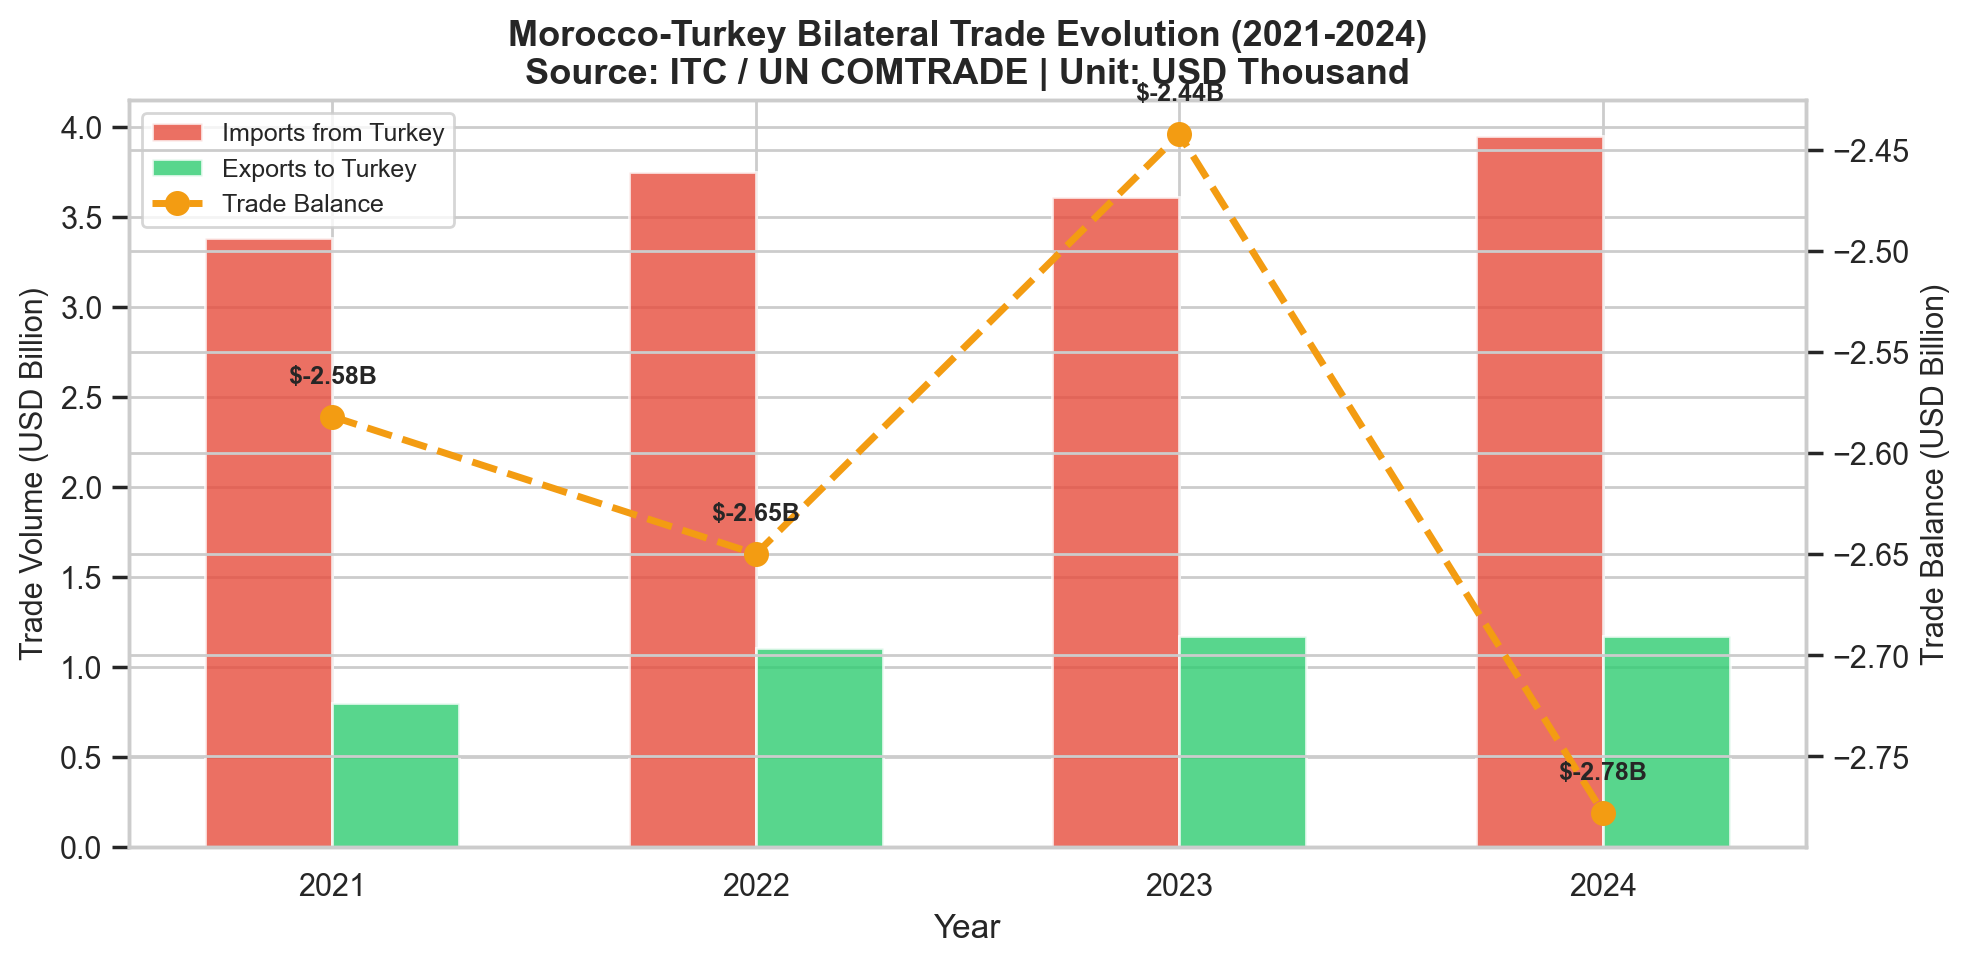
\includegraphics[width=0.95\textwidth]{../charts/01_trade_evolution.png}
\caption{Evolution of bilateral trade between Morocco and Turkey (2021--2024). The persistent gap between imports and exports illustrates the structural trade deficit.}
\end{figure}

The bilateral trade between Morocco and Turkey has grown steadily from 2021 to 2024. However, the gap between imports and exports has remained significant, with Morocco consistently importing more than three times what it exports to Turkey.

\subsection{The ``5-0'' Score Visualization}

\begin{figure}[H]
\centering
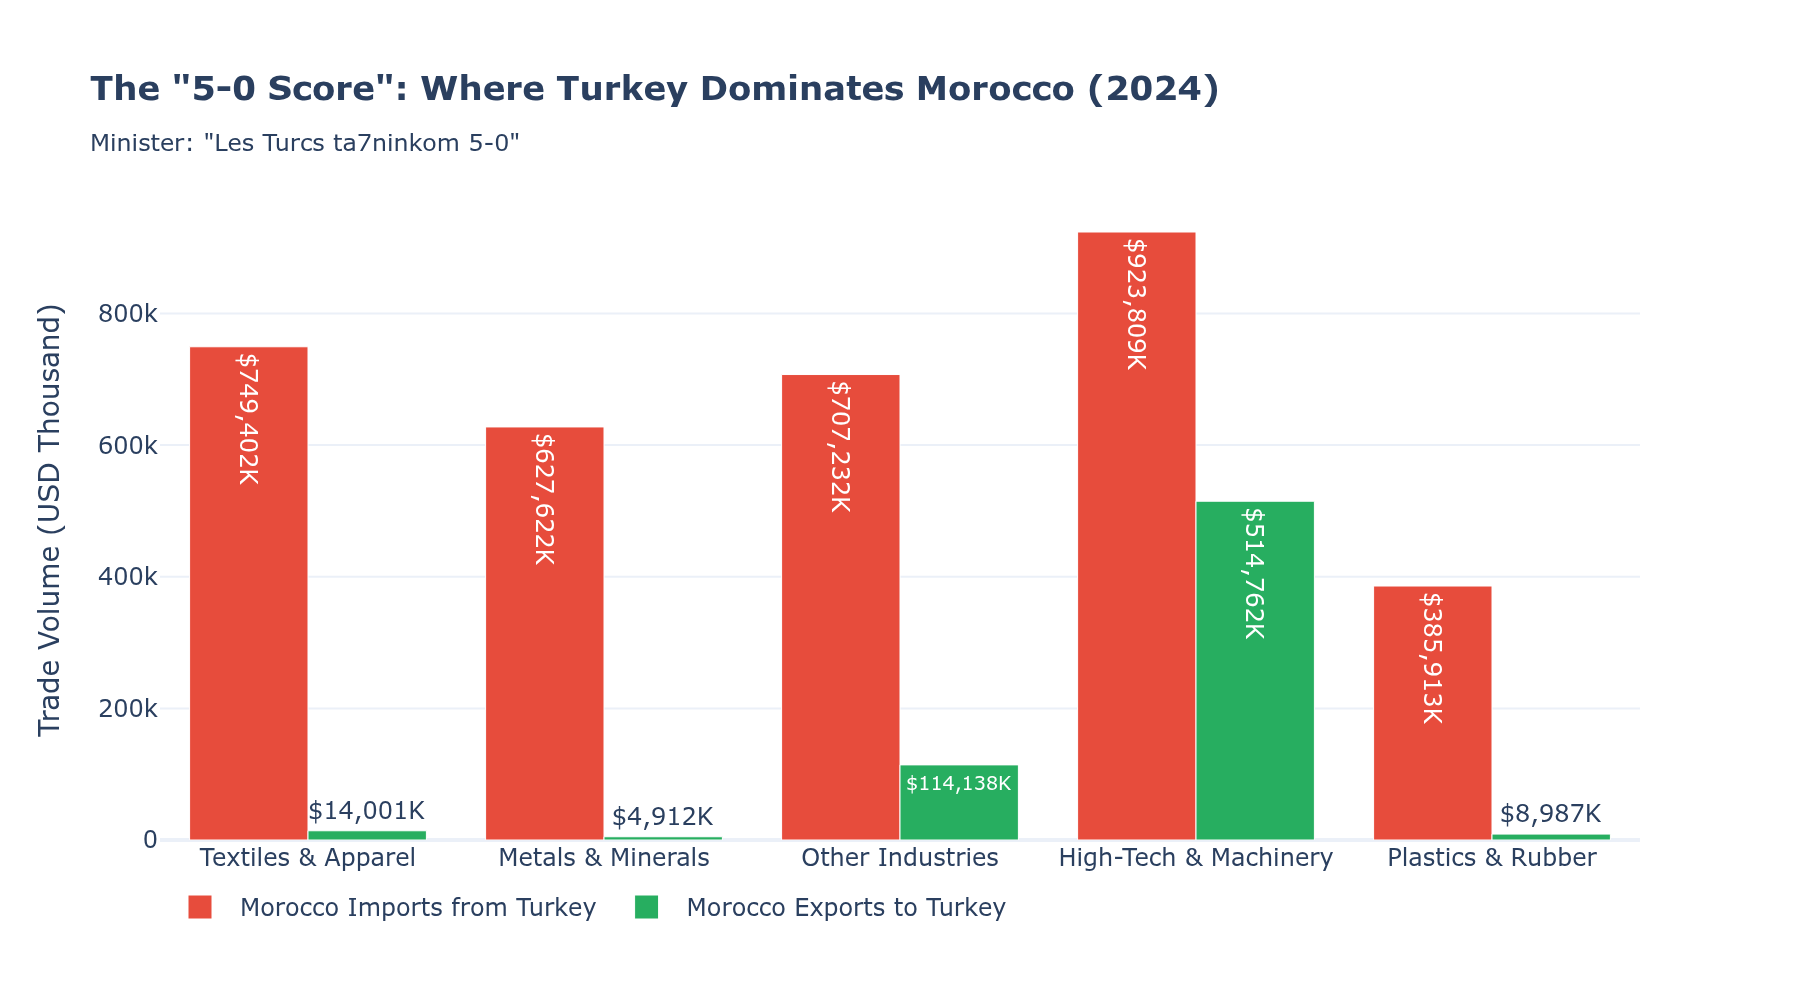
\includegraphics[width=0.95\textwidth]{../charts/03_five_zero_score.png}
\caption{The ``5-0 Score'' --- a visual representation of Turkey's dominance across key trade metrics, inspired by the Minister's metaphor.}
\end{figure}

\subsection{Sector Balance in 2024}

\begin{figure}[H]
\centering
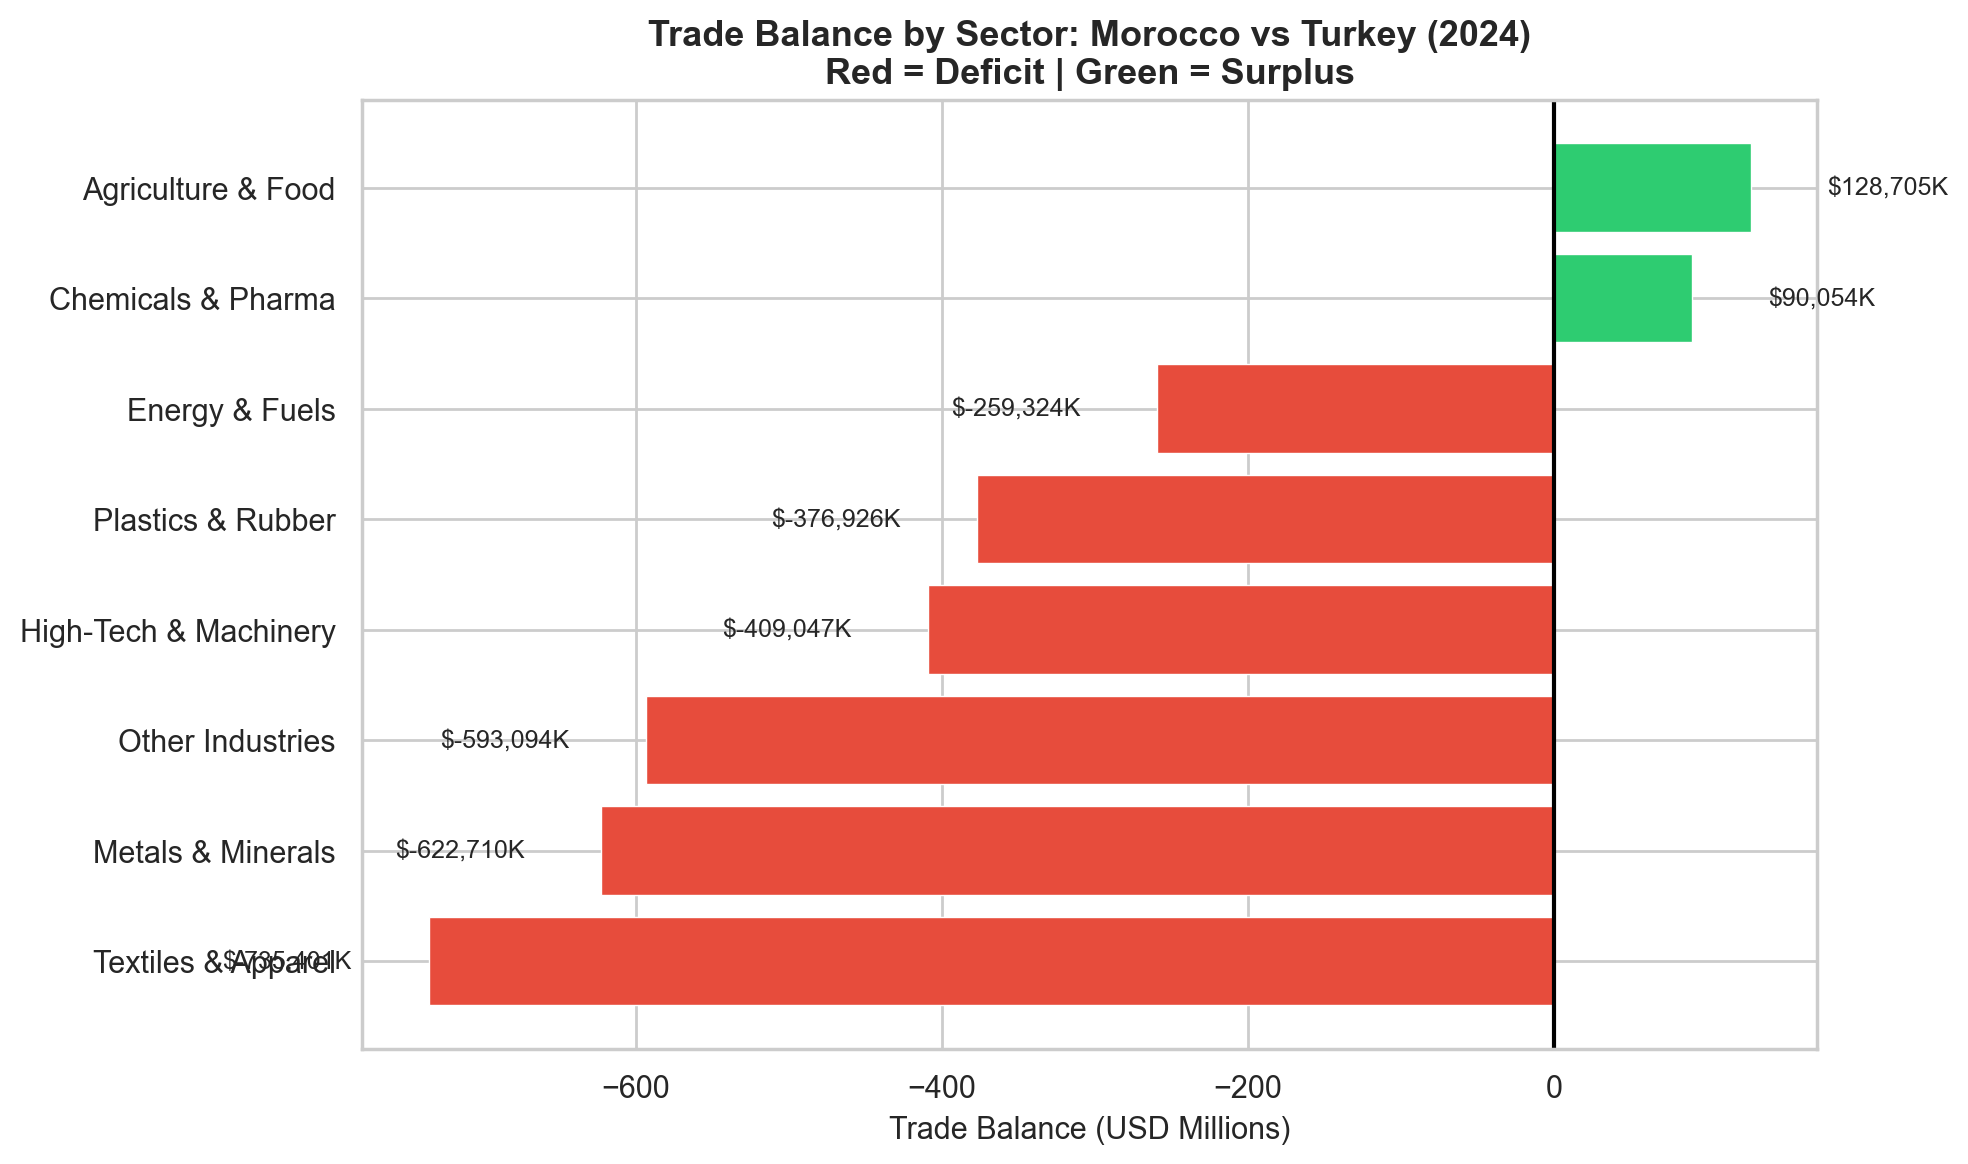
\includegraphics[width=0.95\textwidth]{../charts/02_sector_balance_2024.png}
\caption{Trade balance by sector in 2024. Red sectors indicate trade deficits (Morocco imports more), green sectors indicate surpluses.}
\end{figure}

% ============================================================
% 5. DETAILED SECTOR ANALYSIS
% ============================================================
\section{Detailed Sector Analysis}

\subsection{Sector Performance Summary}

\begin{table}[H]
\centering
\caption{Sector-by-Sector Trade Performance (2024)}
\begin{tabular}{l r r r r}
\toprule
\textbf{Sector} & \textbf{Imports} & \textbf{Exports} & \textbf{Balance} & \textbf{Coverage} \\
 & \textbf{(\$M)} & \textbf{(\$M)} & \textbf{(\$M)} & \textbf{(\%)} \\
\midrule
High-Tech \& Machinery & 923.8 & 514.8 & $-$409.0 & 55.7\% \\
Textiles \& Apparel & 749.4 & 14.0 & $-$735.4 & 1.9\% \\
Other Industries & 707.2 & 114.1 & $-$593.1 & 16.1\% \\
Metals \& Minerals & 627.6 & 4.9 & $-$622.7 & 0.8\% \\
Plastics \& Rubber & 385.9 & 9.0 & $-$376.9 & 2.3\% \\
Energy \& Fuels & 259.4 & 0.1 & $-$259.3 & 0.04\% \\
Chemicals \& Pharma & 188.6 & 278.6 & +90.1 & 147.8\% \\
Agriculture \& Food & 107.8 & 236.5 & +128.7 & 219.4\% \\
\midrule
\textbf{Total} & \textbf{3,949.8} & \textbf{1,172.0} & \textbf{$-$2,777.5} & \textbf{29.7\%} \\
\bottomrule
\end{tabular}
\end{table}

\subsection{Key Observations by Sector}

\subsubsection{Deficit Sectors (Morocco imports more)}

\begin{itemize}
\item \textbf{Textiles \& Apparel} ($-$\$735M): The largest deficit sector. Turkey dominates with its vertically integrated textile industry. Coverage ratio is only 1.9\%.
\item \textbf{Metals \& Minerals} ($-$\$623M): Heavy dependence on Turkish steel and metal products.
\item \textbf{Other Industries} ($-$\$593M): Diverse products where Turkey has established manufacturing capacity.
\item \textbf{High-Tech \& Machinery} ($-$\$409M): Despite the deficit, this sector shows the strongest export CAGR of 33.1\%, indicating rapid improvement.
\item \textbf{Plastics \& Rubber} ($-$\$377M): Growing imports (CAGR +13.8\%) outpacing modest export growth.
\item \textbf{Energy \& Fuels} ($-$\$259M): Near-zero exports; the fastest-growing import sector (CAGR +97.8\%).
\end{itemize}

\subsubsection{Surplus Sectors (Morocco exports more)}

\begin{itemize}
\item \textbf{Agriculture \& Food} (+\$129M): Morocco's strongest sector with a coverage ratio of 219\%, leveraging its agricultural comparative advantage.
\item \textbf{Chemicals \& Pharma} (+\$90M): Coverage ratio of 148\%, driven by phosphate-based chemical exports.
\end{itemize}

\subsection{Deficit Evolution Over Time}

\begin{figure}[H]
\centering
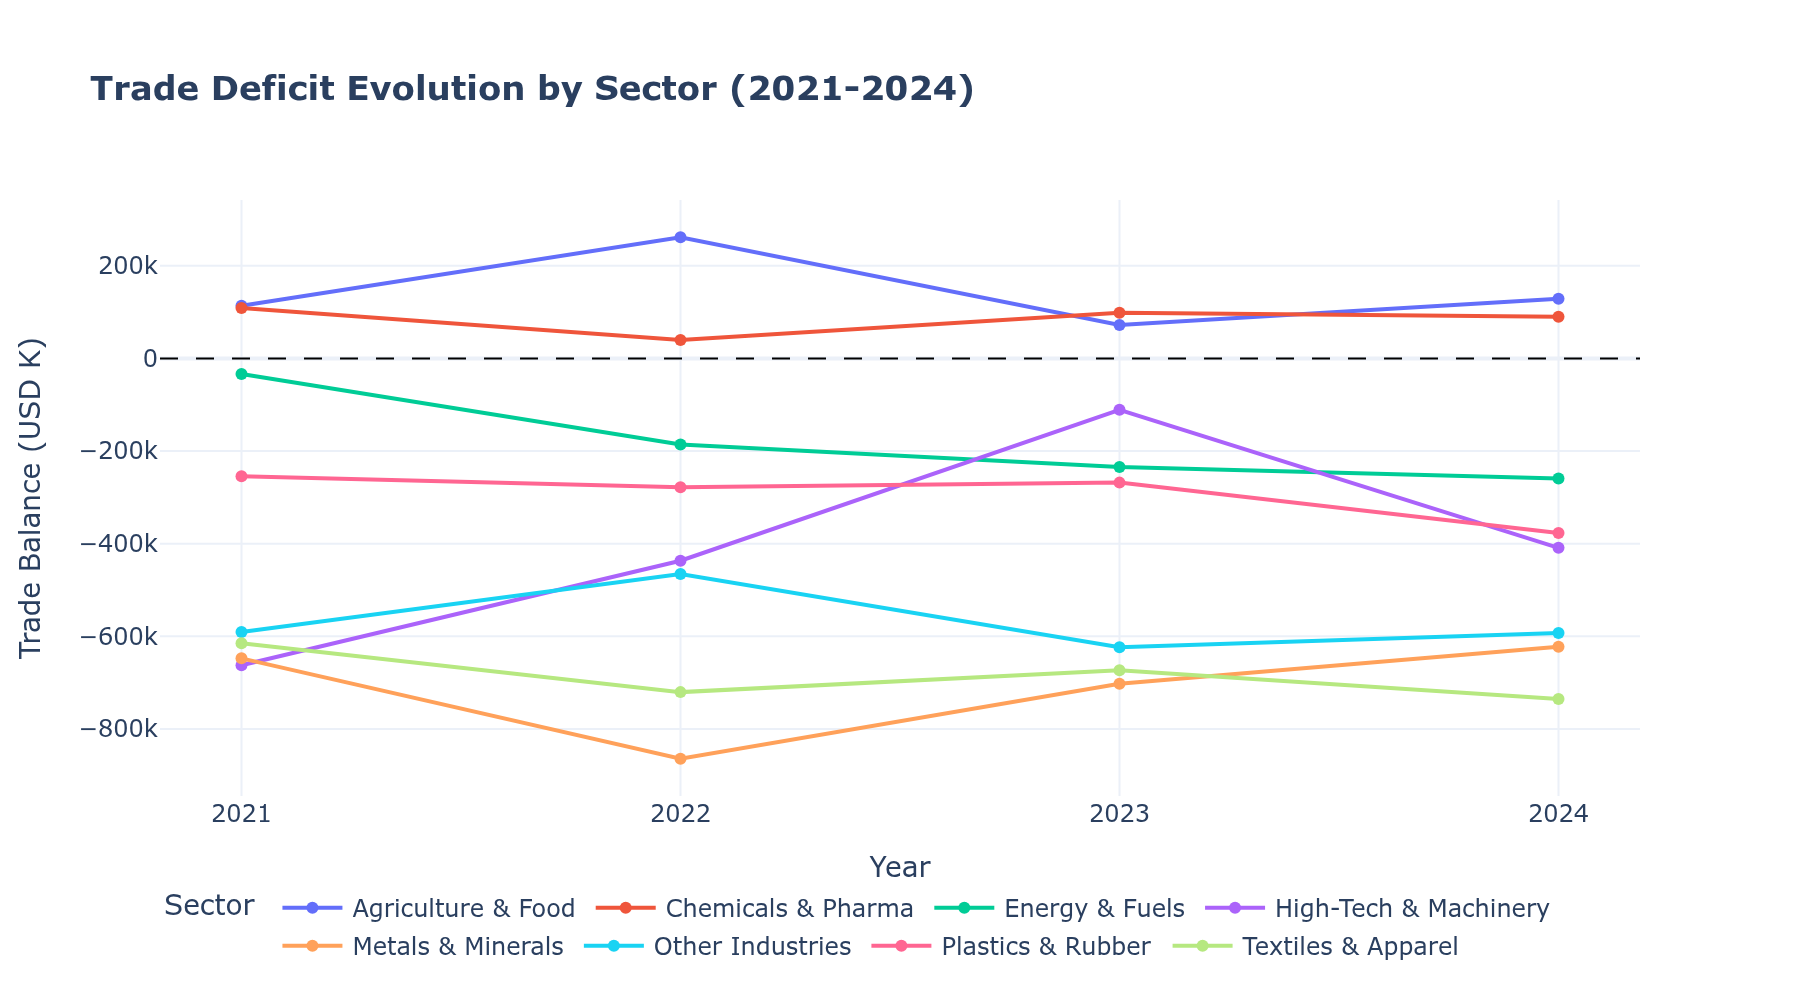
\includegraphics[width=0.95\textwidth]{../charts/04_deficit_evolution.png}
\caption{Evolution of the trade deficit from 2021 to 2024, showing the structural nature of the imbalance.}
\end{figure}

\subsection{Trade Balance Heatmap}

\begin{figure}[H]
\centering
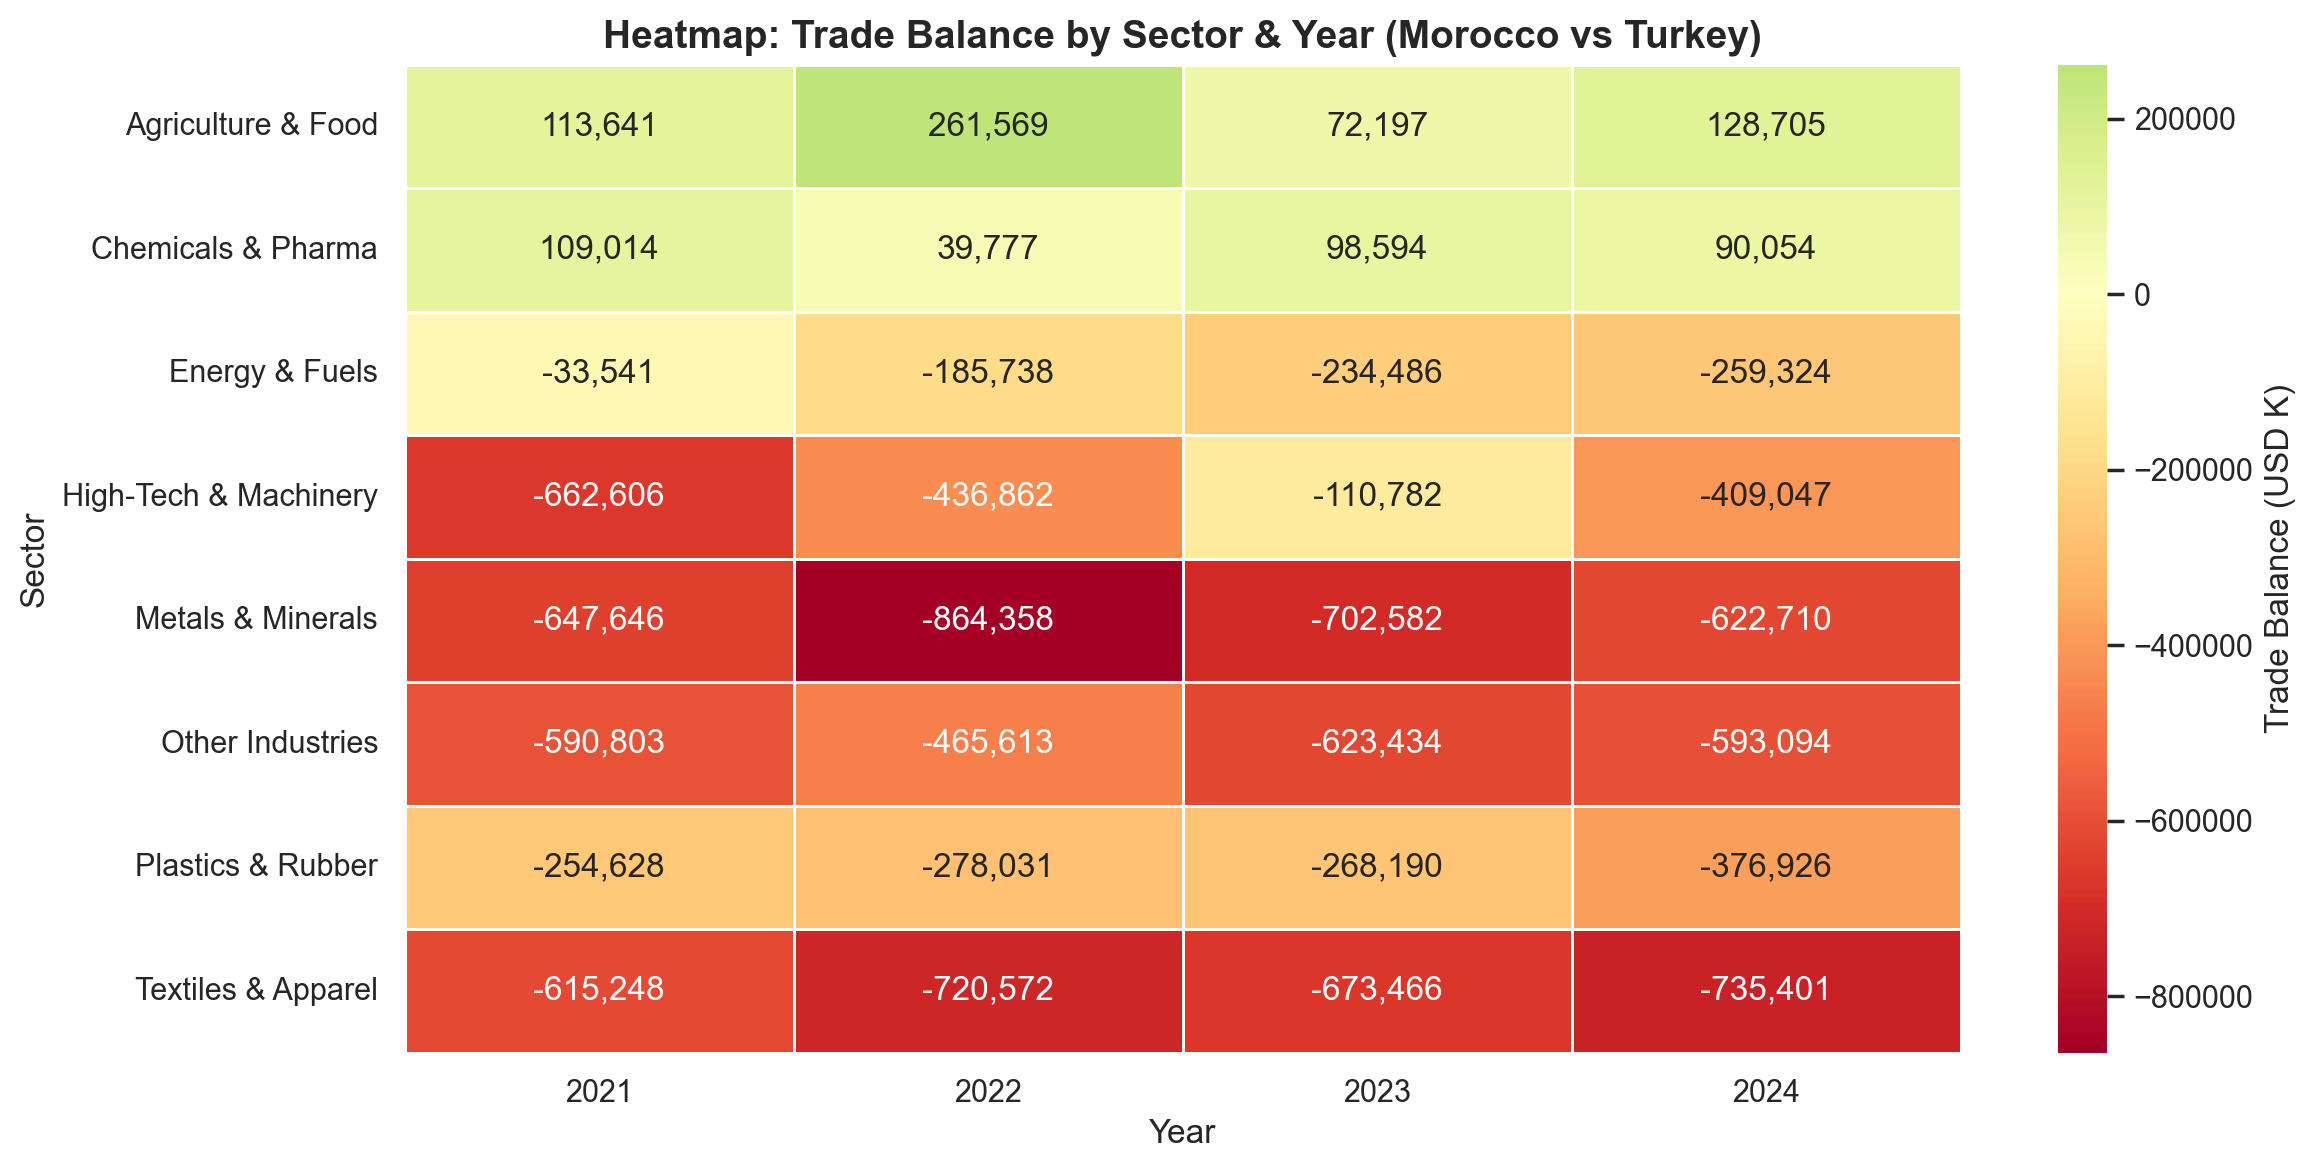
\includegraphics[width=0.95\textwidth]{../charts/05_heatmap_balance.png}
\caption{Heatmap of trade balance by product and year. Red cells indicate deficits, green cells indicate surpluses.}
\end{figure}

% ============================================================
% 6. TOP PRODUCTS ANALYSIS
% ============================================================
\section{Top Products Analysis}

\subsection{Top 10 Deficit Products}

\begin{figure}[H]
\centering
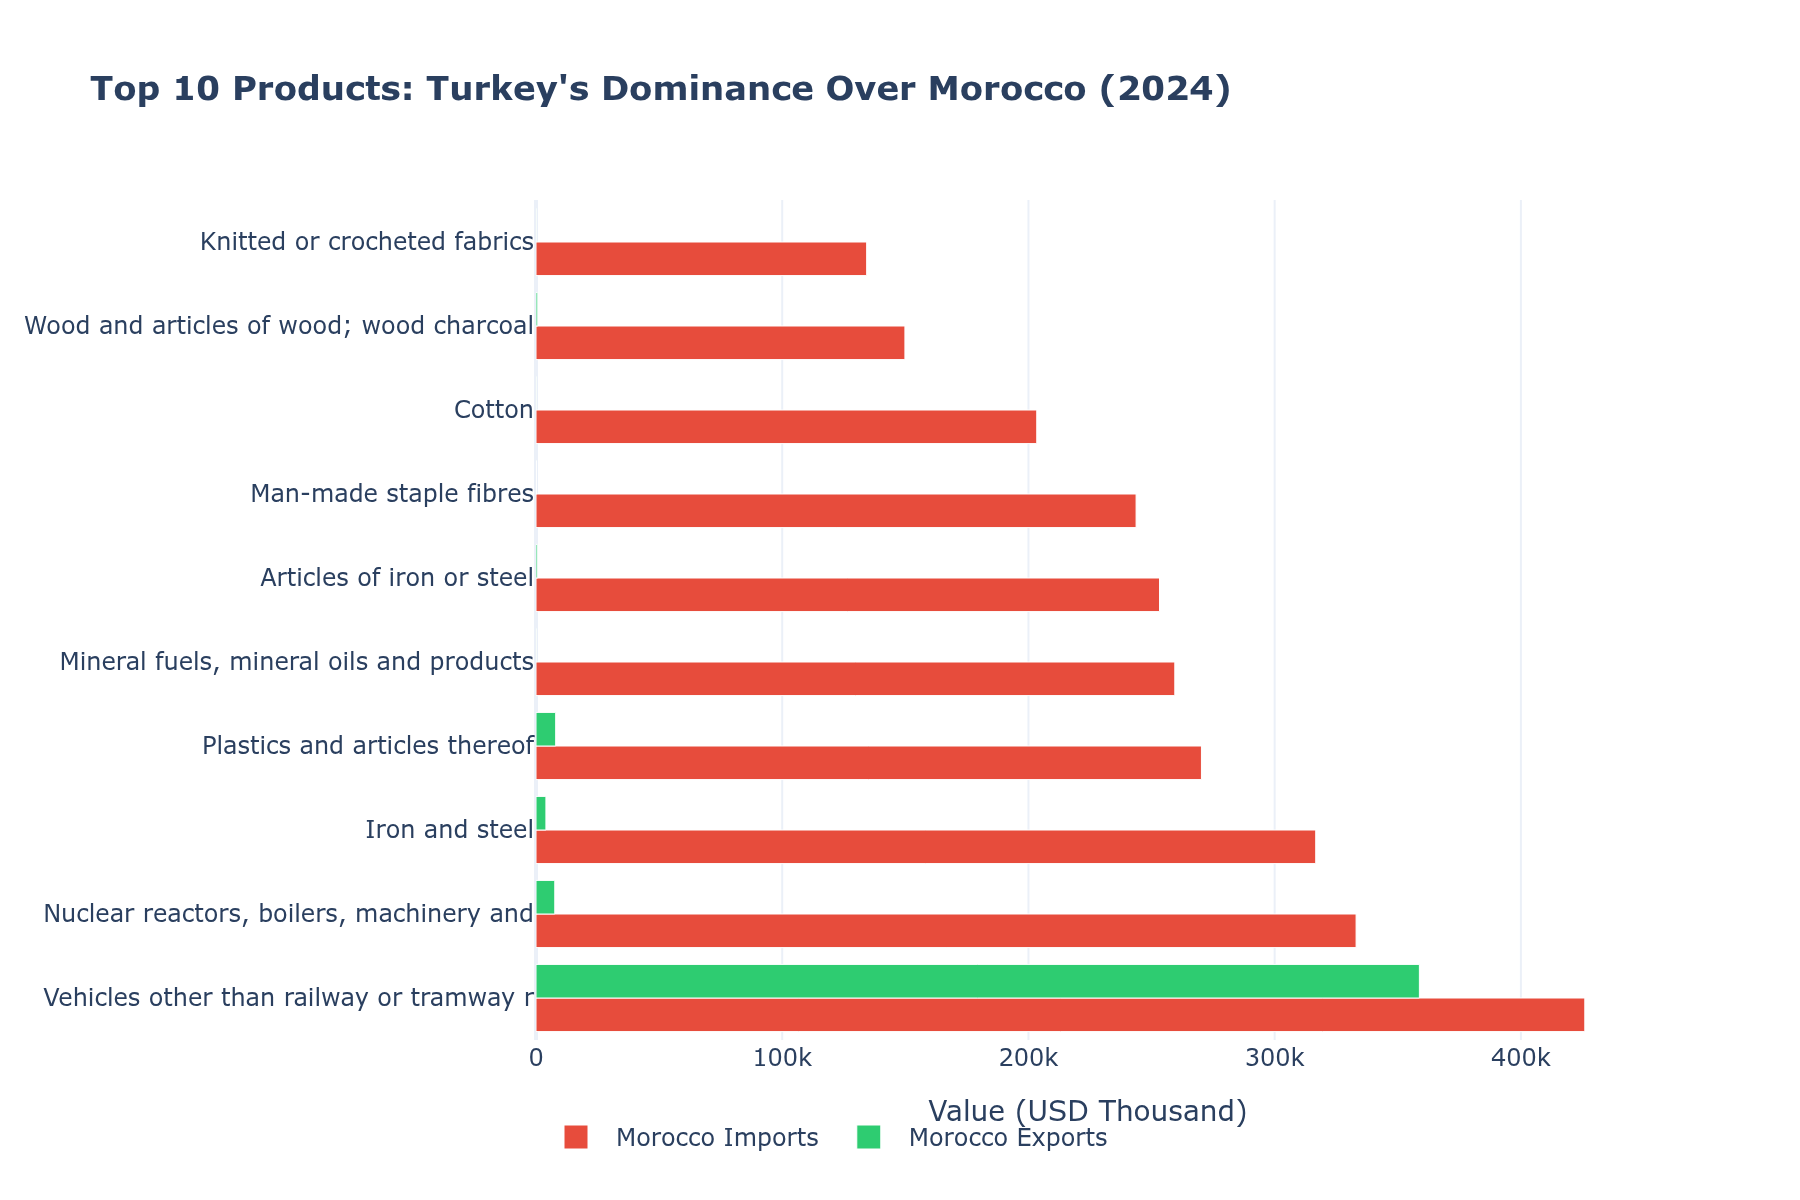
\includegraphics[width=0.95\textwidth]{../charts/06_top10_deficit_products.png}
\caption{The 10 product categories with the largest trade deficits in 2024. These products drive Morocco's trade imbalance with Turkey.}
\end{figure}

\subsection{Top 10 Surplus Products}

\begin{figure}[H]
\centering
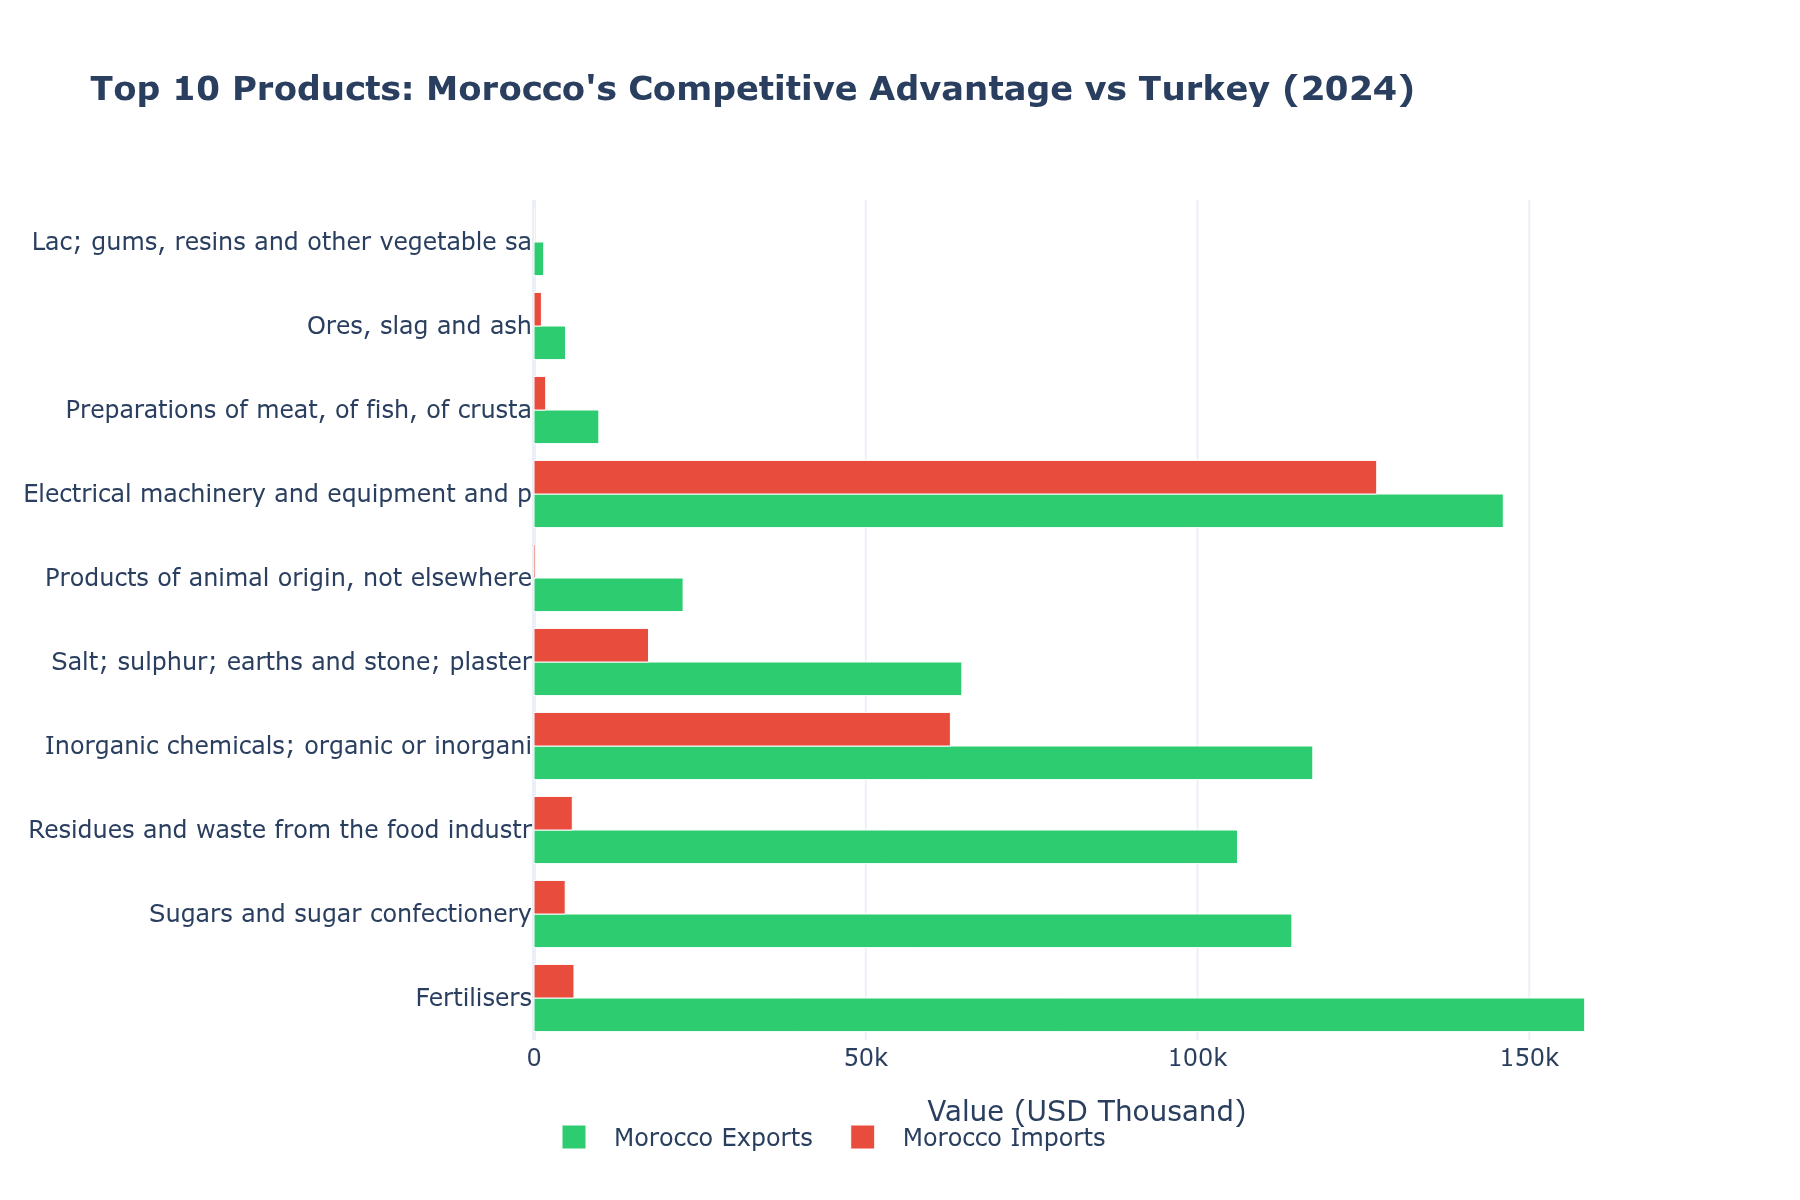
\includegraphics[width=0.95\textwidth]{../charts/07_top10_surplus_products.png}
\caption{The 10 product categories where Morocco maintains a trade surplus with Turkey. Agriculture and chemicals dominate.}
\end{figure}

\subsection{Import and Export Composition}

\begin{figure}[H]
\centering
\begin{subfigure}{0.48\textwidth}
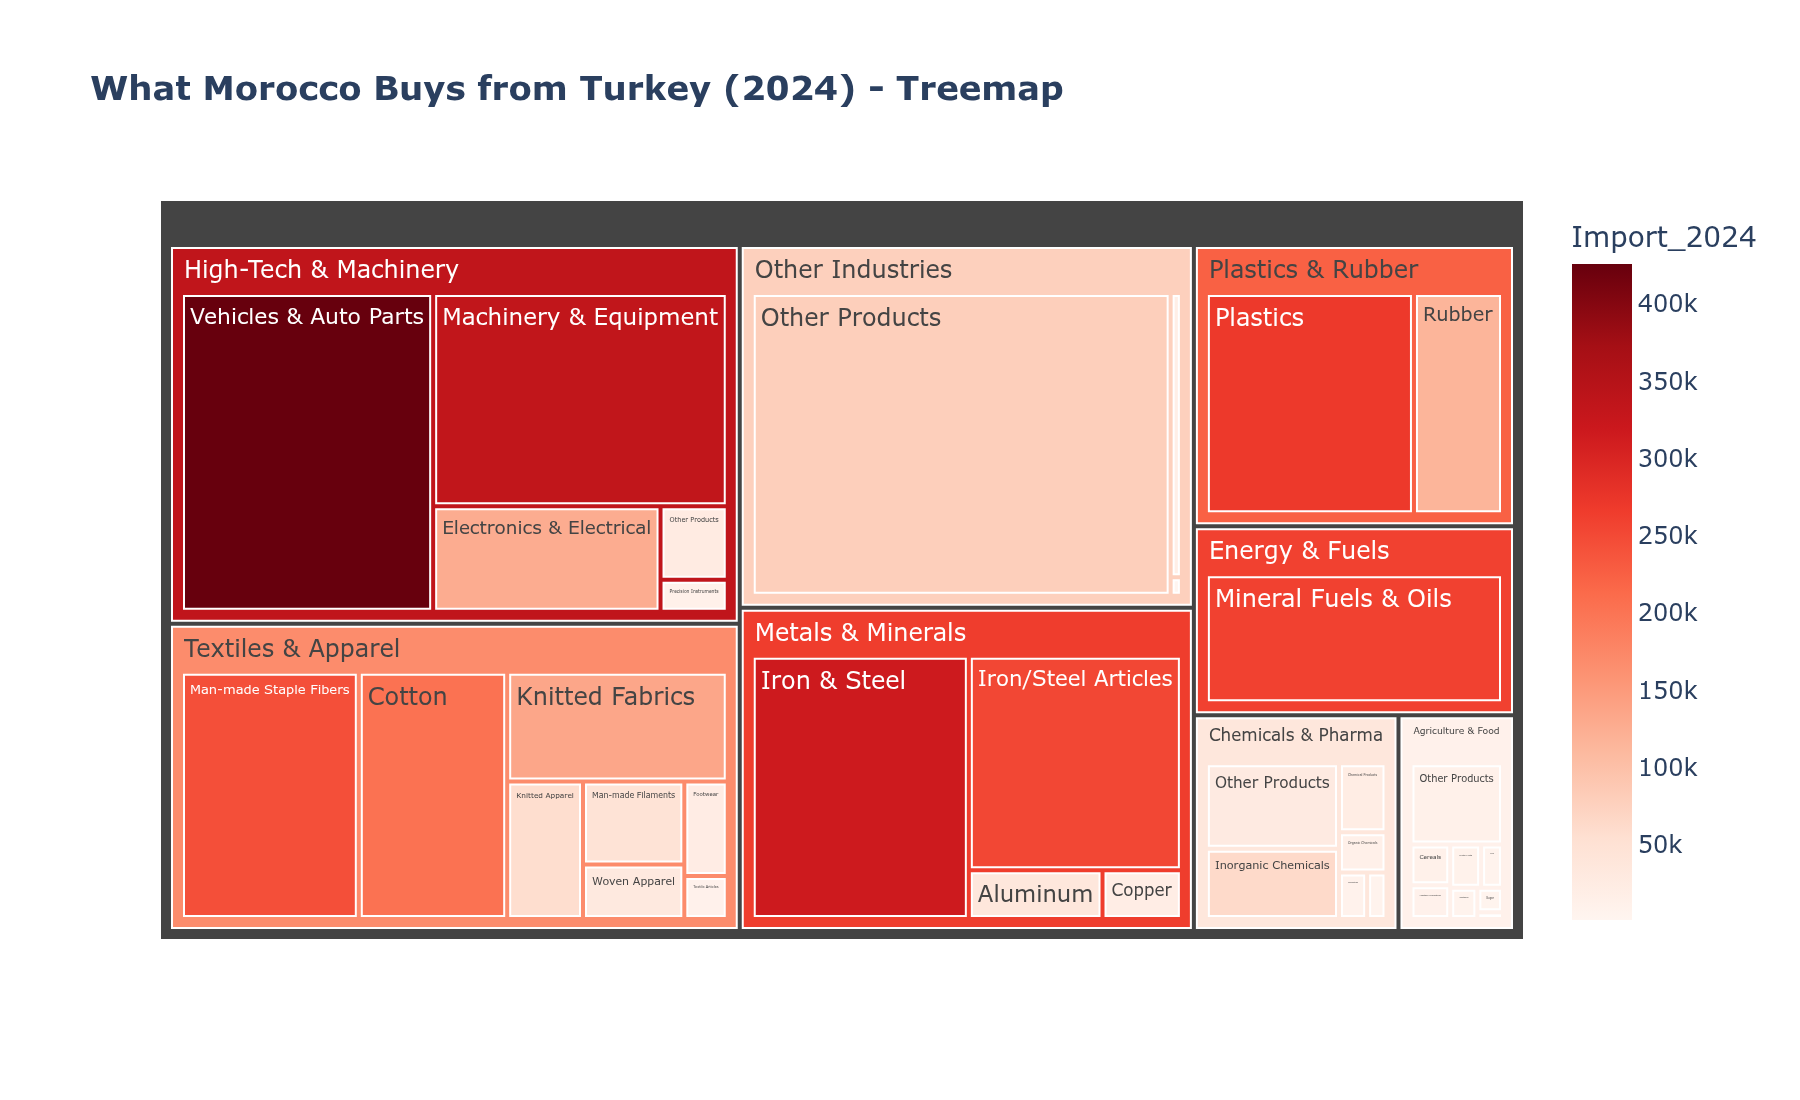
\includegraphics[width=\textwidth]{../charts/10_treemap_imports.png}
\caption{Import treemap}
\end{subfigure}
\hfill
\begin{subfigure}{0.48\textwidth}
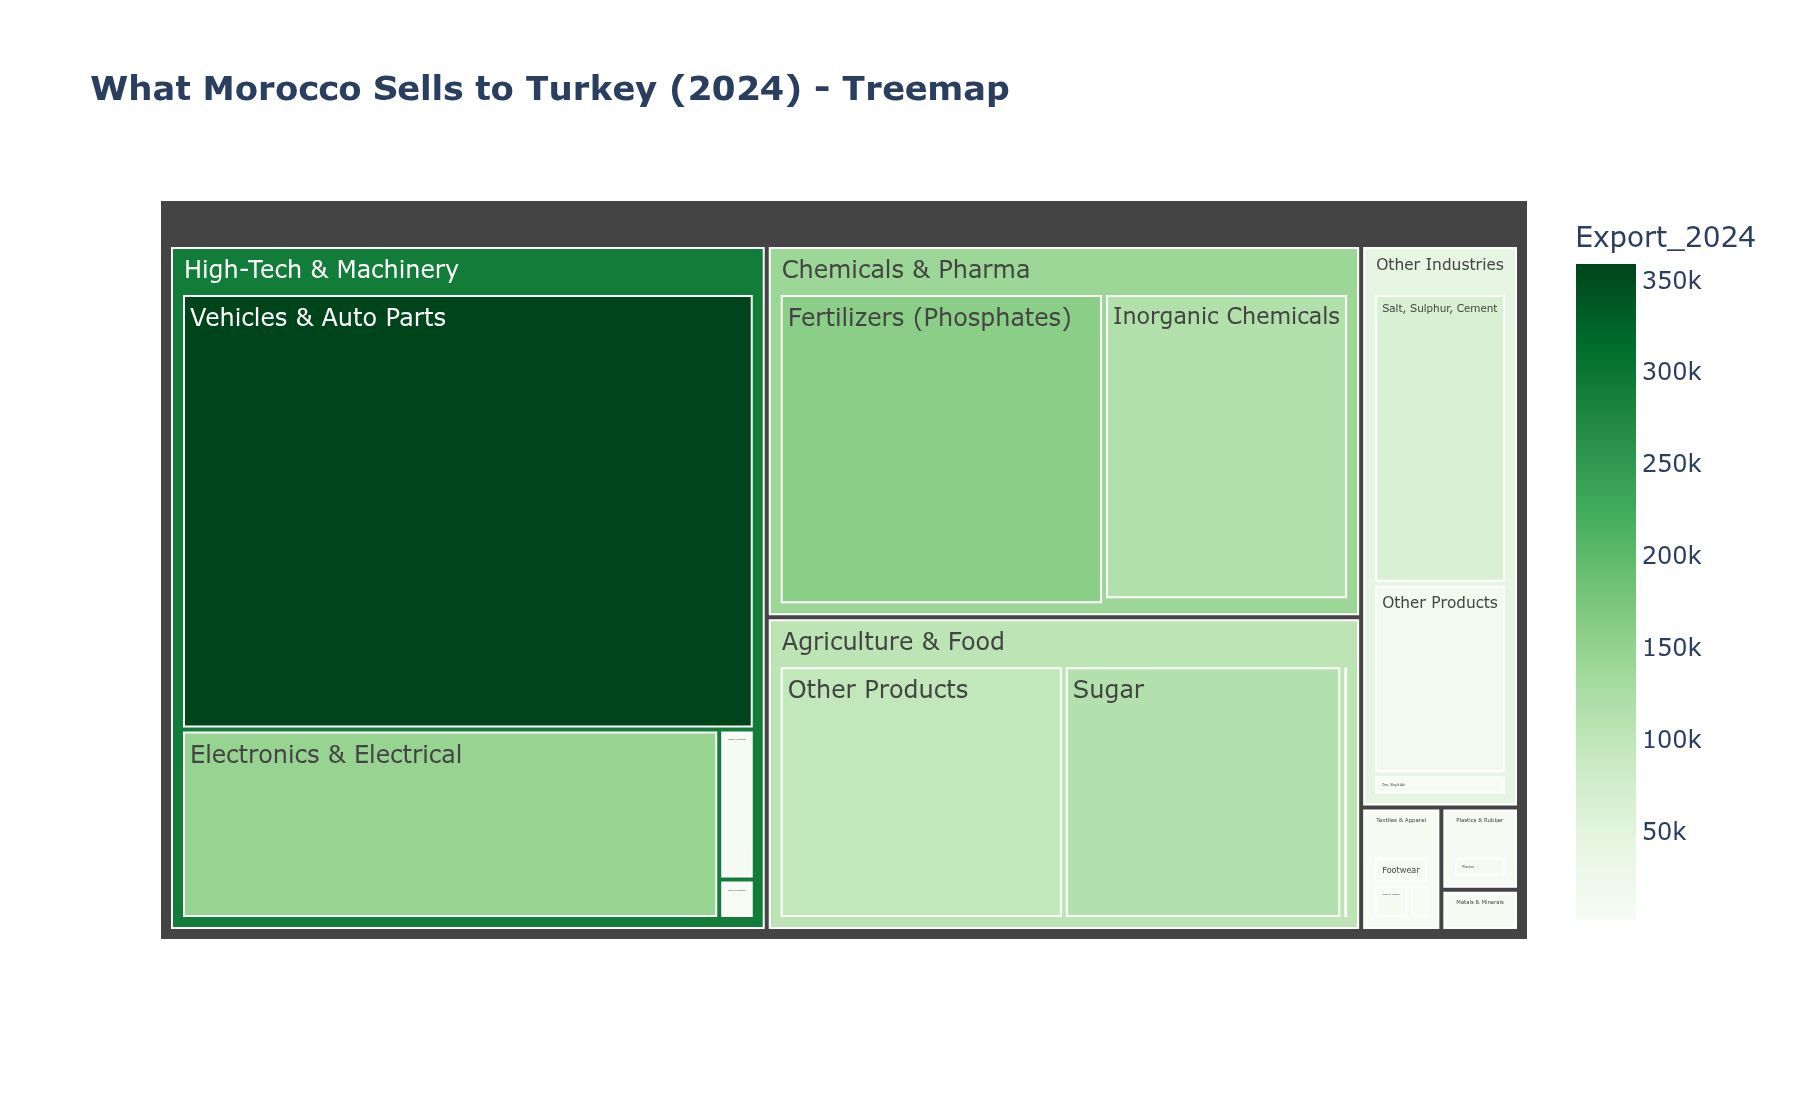
\includegraphics[width=\textwidth]{../charts/11_treemap_exports.png}
\caption{Export treemap}
\end{subfigure}
\caption{Treemap visualization of import (left) and export (right) composition by product category. The size of each rectangle represents the trade value.}
\end{figure}

\begin{figure}[H]
\centering
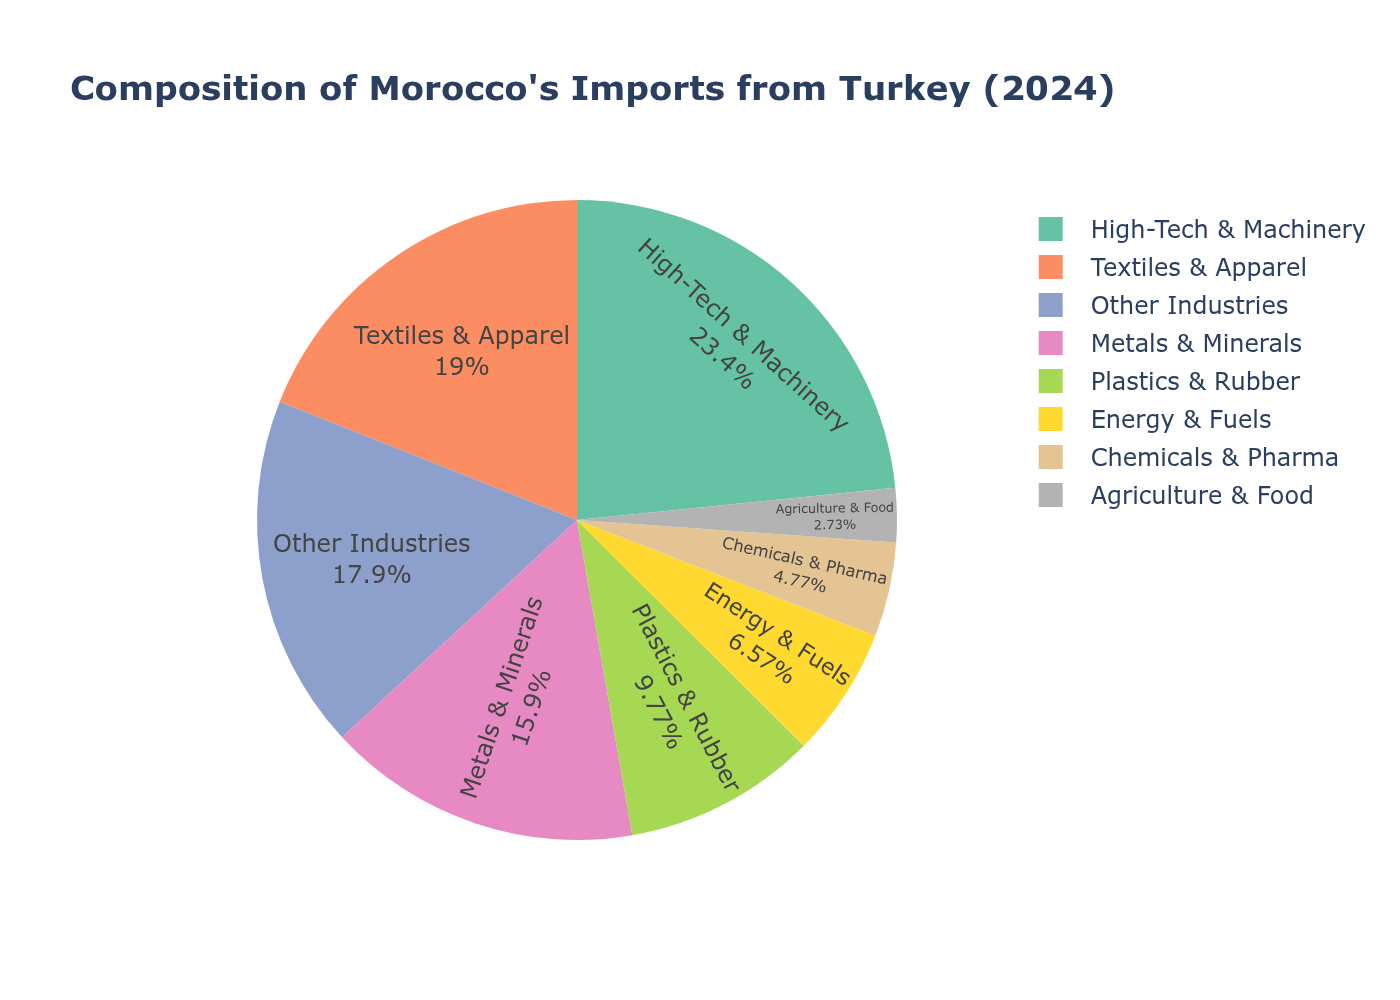
\includegraphics[width=0.85\textwidth]{../charts/14_import_composition_pie.png}
\caption{Pie chart breakdown of Morocco's import composition from Turkey by sector.}
\end{figure}

% ============================================================
% 7. GROWTH ANALYSIS (CAGR)
% ============================================================
\section{Growth Analysis (CAGR 2021--2024)}

\subsection{Overall Growth Trends}

Morocco's exports to Turkey are growing at a CAGR of \textbf{13.6\%}, significantly outpacing import growth of \textbf{5.3\%}. If this trend continues, the coverage ratio will improve over time, though it will take many years to close the gap at current rates.

\subsection{Sector-Level CAGR}

\begin{figure}[H]
\centering
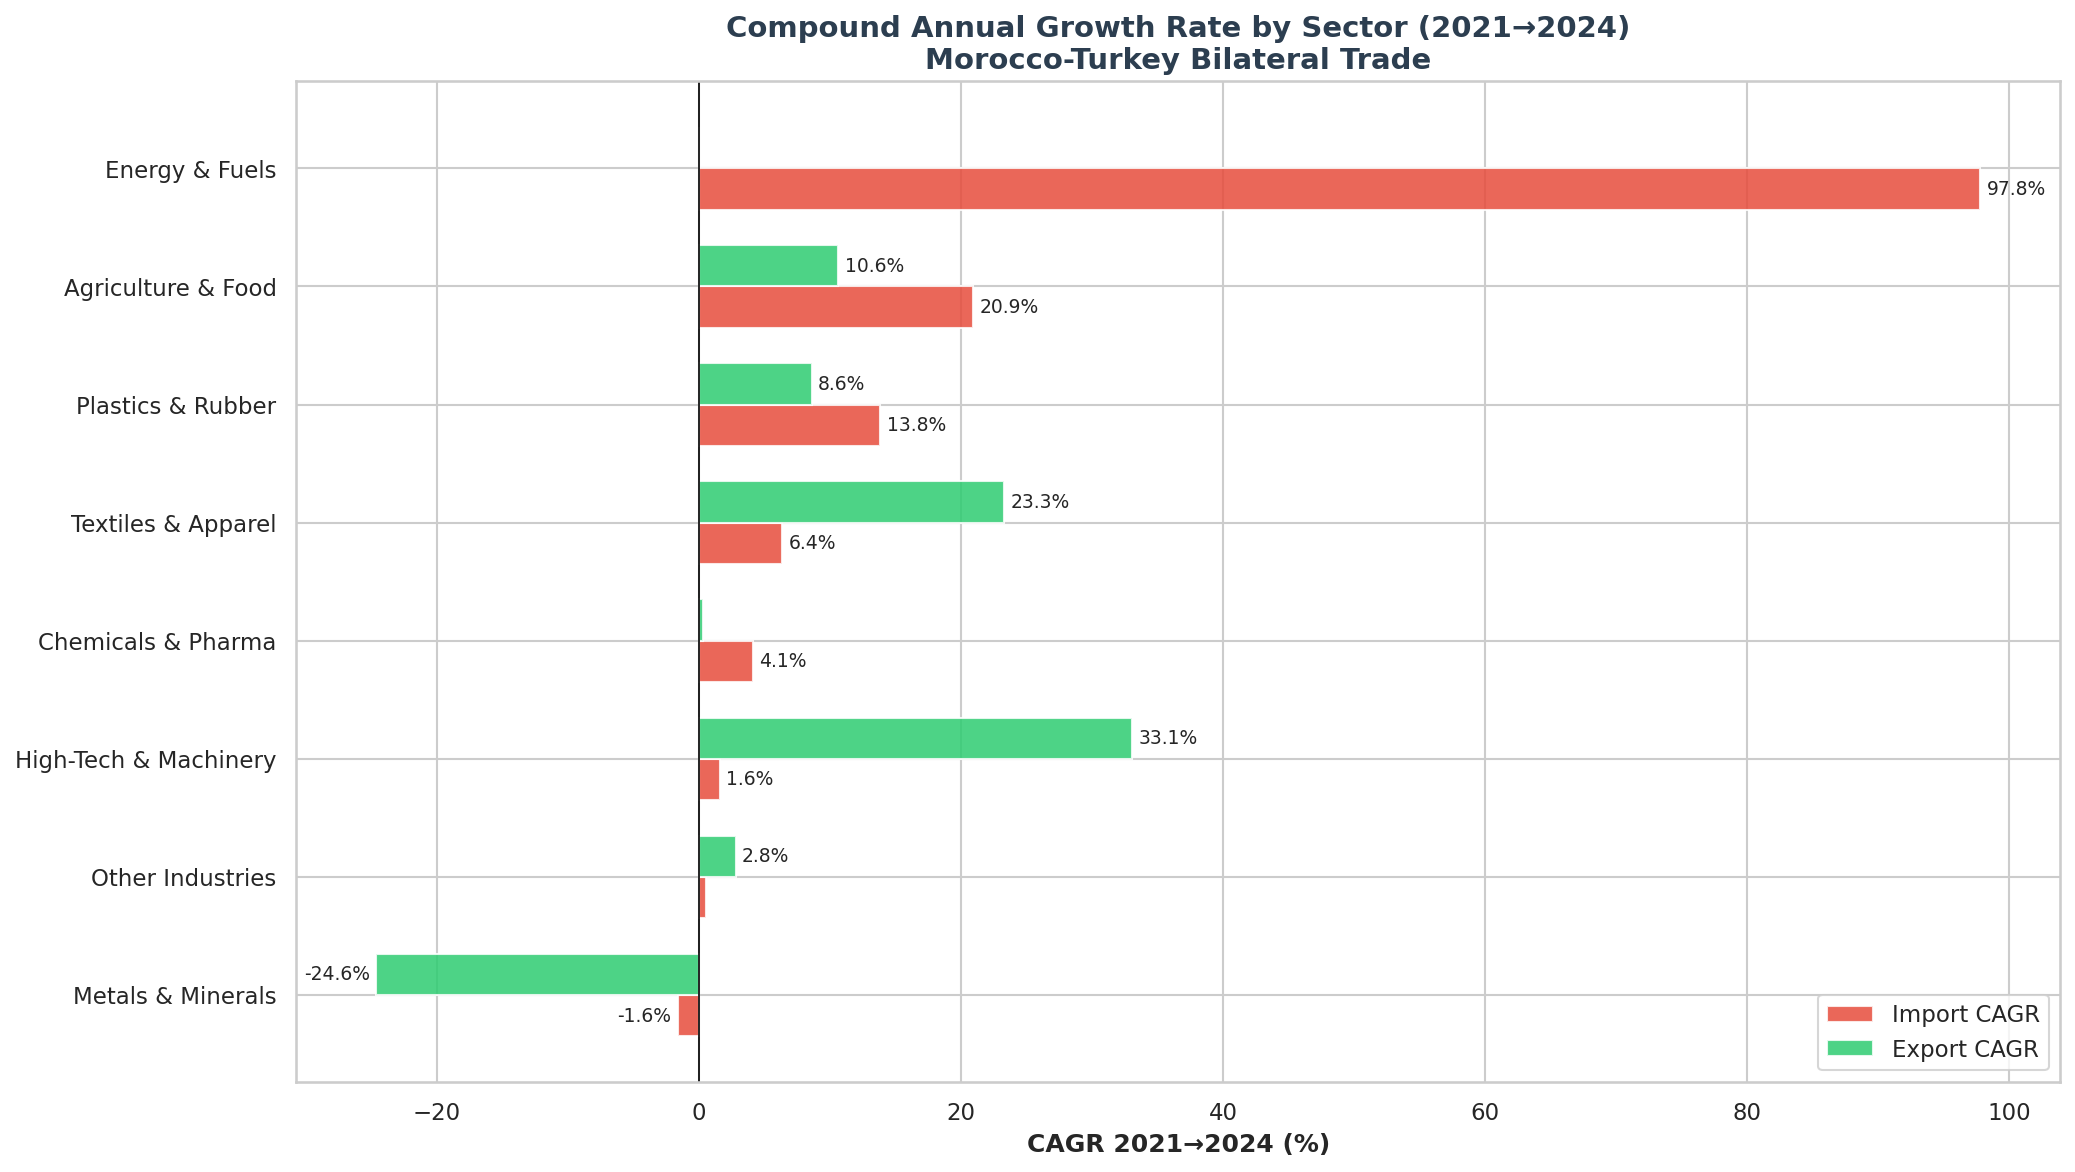
\includegraphics[width=0.95\textwidth]{../charts/17_cagr_by_sector.png}
\caption{Compound Annual Growth Rate (2021$\rightarrow$2024) by sector. Green bars show export growth, red bars show import growth.}
\end{figure}

\begin{table}[H]
\centering
\caption{CAGR by Sector (2021$\rightarrow$2024)}
\begin{tabular}{l r r l}
\toprule
\textbf{Sector} & \textbf{Import CAGR} & \textbf{Export CAGR} & \textbf{Trend} \\
\midrule
Energy \& Fuels & +97.8\% & 0.0\% & Rapidly widening \\
Agriculture \& Food & +20.9\% & +10.6\% & Import growing faster \\
Plastics \& Rubber & +13.8\% & +8.6\% & Import growing faster \\
Textiles \& Apparel & +6.4\% & +23.3\% & Export catching up \\
Chemicals \& Pharma & +4.1\% & +0.3\% & Stable surplus \\
High-Tech \& Machinery & +1.6\% & +33.1\% & Export surging \\
Other Industries & +0.5\% & +2.8\% & Slow improvement \\
Metals \& Minerals & $-$1.6\% & $-$24.6\% & Both declining \\
\bottomrule
\end{tabular}
\end{table}

\subsection{Growth Comparison}

\begin{figure}[H]
\centering
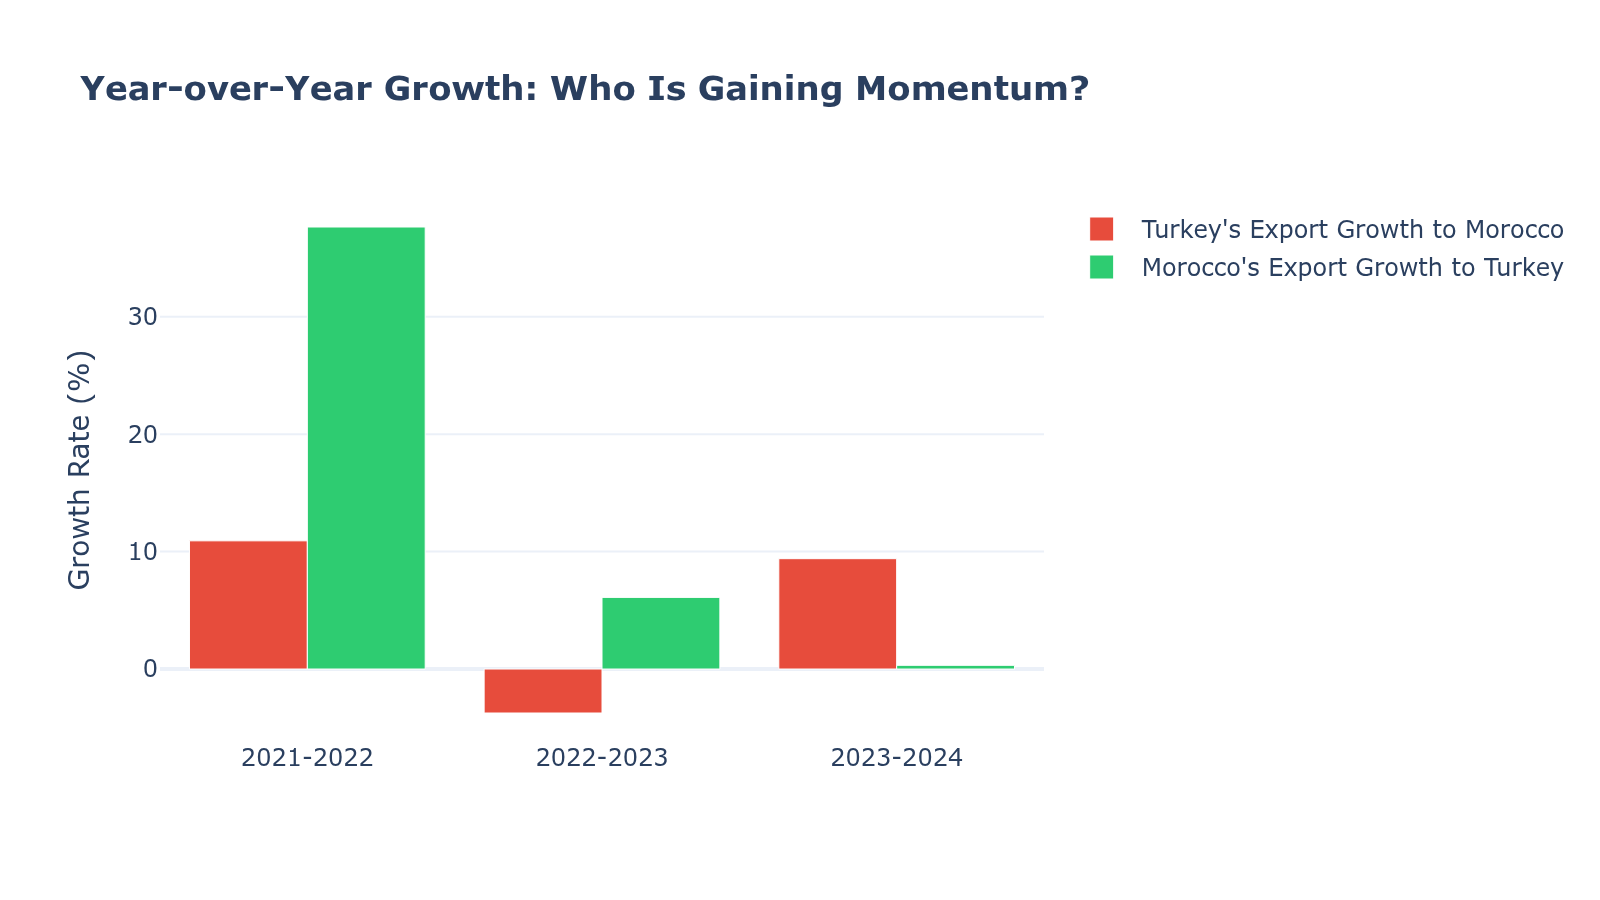
\includegraphics[width=0.95\textwidth]{../charts/09_growth_comparison.png}
\caption{Year-over-year growth comparison of imports vs exports, highlighting divergent trends.}
\end{figure}

% ============================================================
% 8. ADVANCED METRICS
% ============================================================
\section{Advanced Metrics}

\subsection{Market Concentration (HHI)}

\begin{figure}[H]
\centering
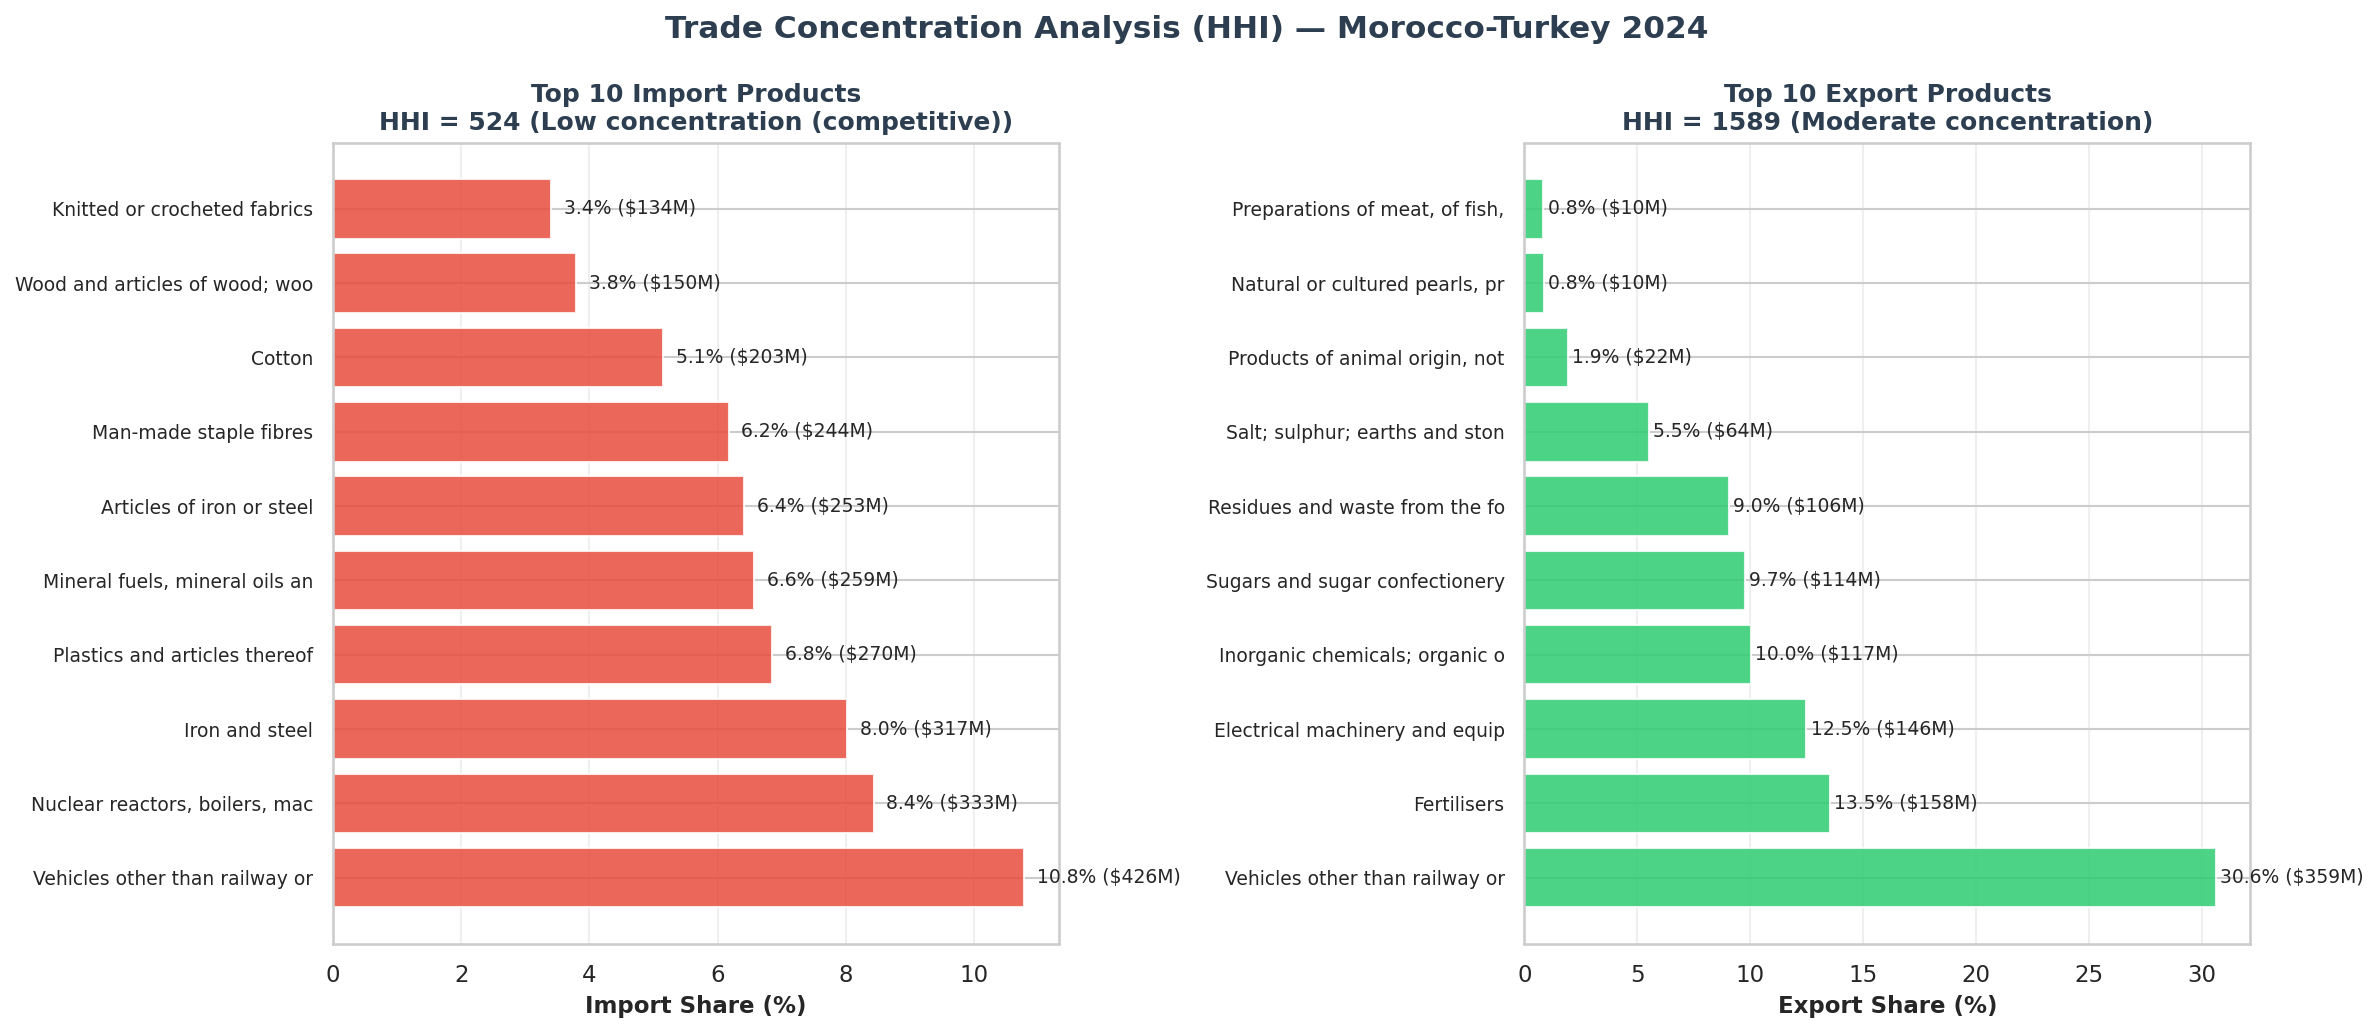
\includegraphics[width=0.95\textwidth]{../charts/21_hhi_concentration.png}
\caption{HHI concentration analysis showing the distribution of trade across product categories.}
\end{figure}

\textbf{Key insight:} Morocco's imports from Turkey (HHI = 524) are highly diversified across many products, while exports (HHI = 1,589) are moderately concentrated, indicating dependency on fewer product categories.

This asymmetry is problematic: Turkey sells a wide range of products to Morocco, but Morocco's export basket to Turkey relies heavily on a smaller number of products, mainly in agriculture and chemicals.

\subsection{Revealed Comparative Advantage (RCA)}

Morocco has a revealed comparative advantage (RCA $>$ 1) in \textbf{14 product categories}. The strongest RCA sectors are:

\begin{itemize}
\item \textbf{Agriculture \& Food}: Leveraging Morocco's Mediterranean climate and OCP Group's phosphate-based fertilizers
\item \textbf{Chemicals \& Pharma}: Driven by the world's largest phosphate reserves
\item \textbf{Automotive components}: Emerging sector with growing RCA thanks to the Tangier automotive hub
\end{itemize}

\subsection{Dependency Index and Coverage}

\begin{figure}[H]
\centering
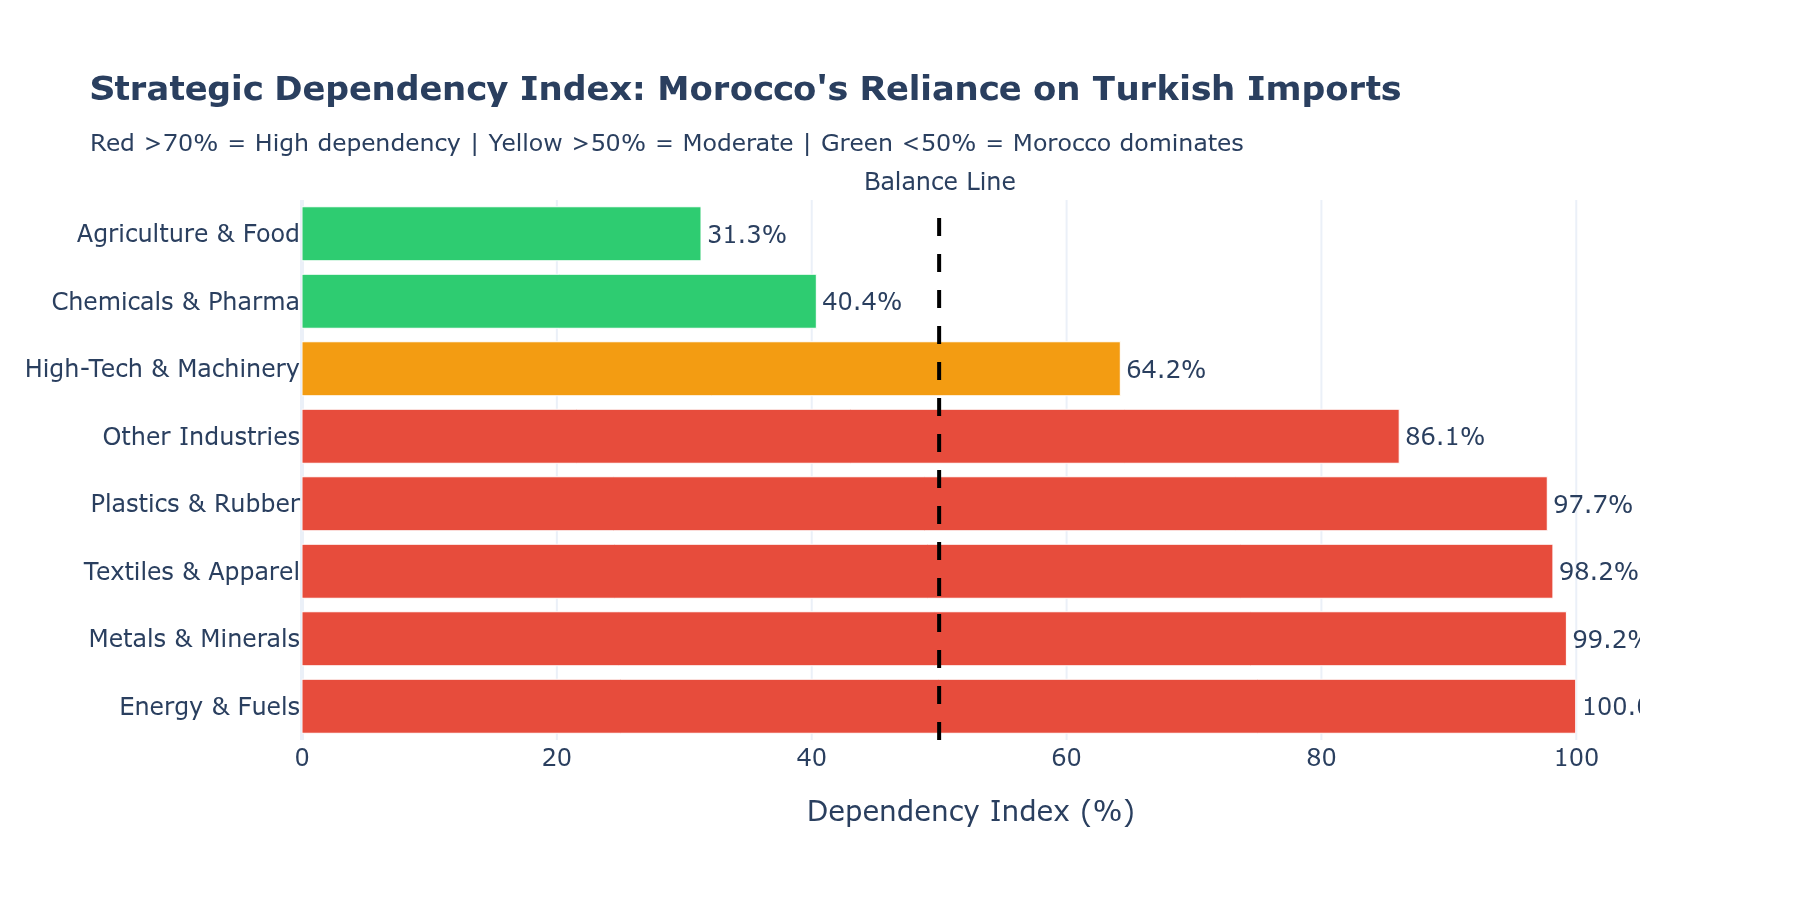
\includegraphics[width=0.95\textwidth]{../charts/12_dependency_index.png}
\caption{Morocco's trade dependency index by sector, showing the degree of reliance on Turkish imports.}
\end{figure}

\begin{figure}[H]
\centering
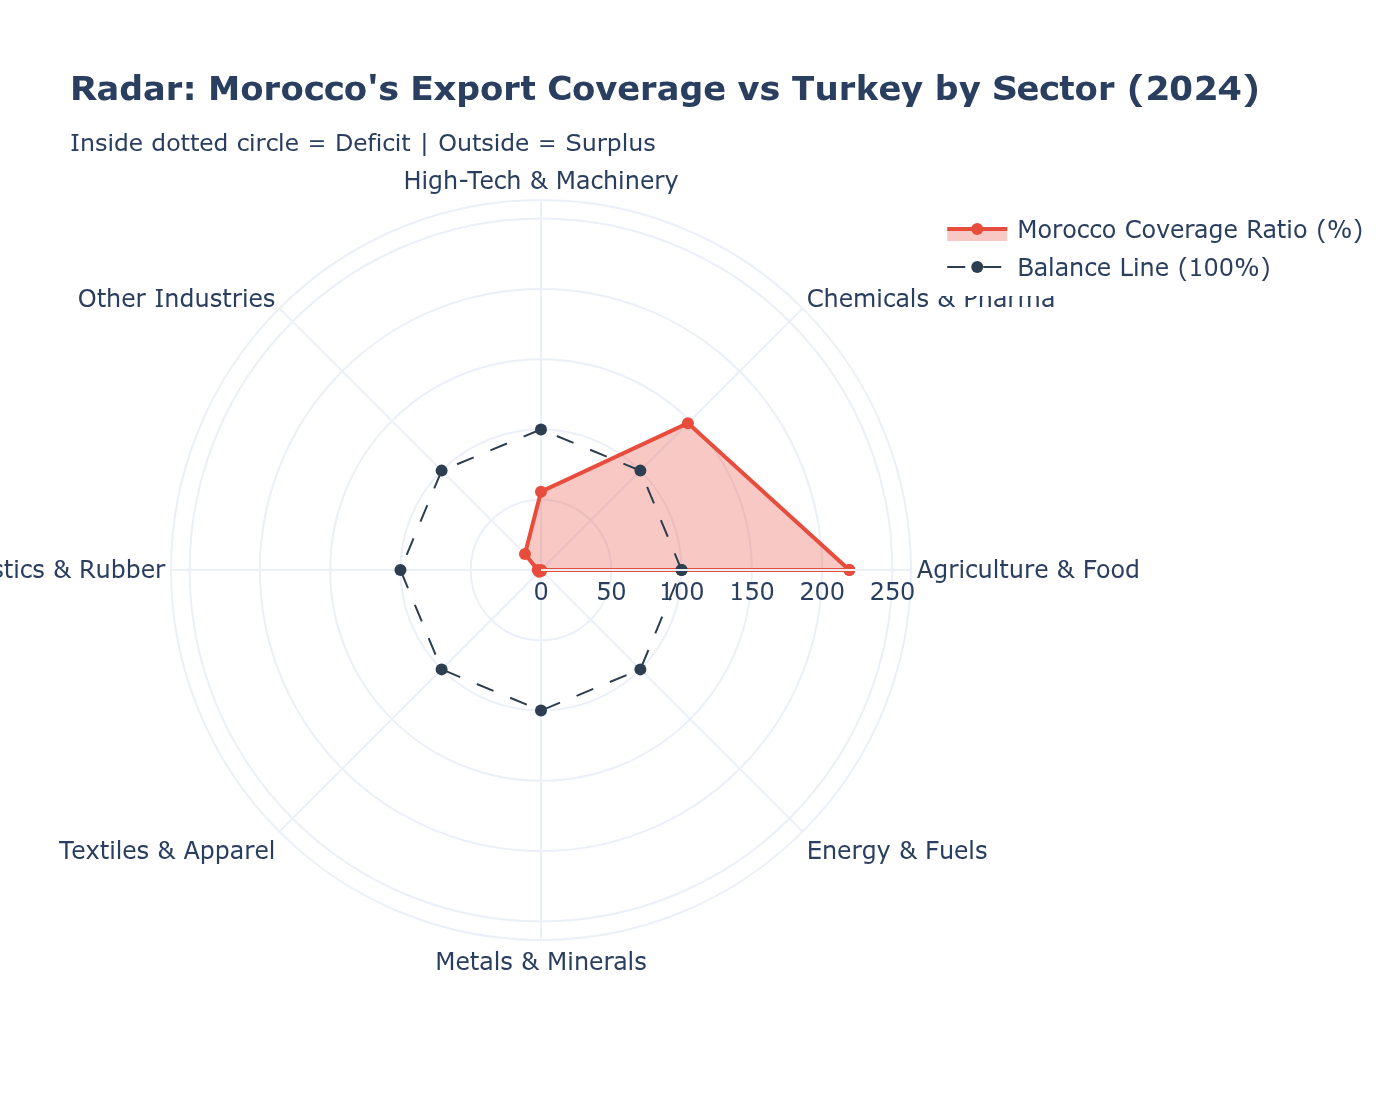
\includegraphics[width=0.95\textwidth]{../charts/08_radar_coverage.png}
\caption{Radar chart of export coverage ratio by sector. Values closer to the outer edge indicate better coverage.}
\end{figure}

% ============================================================
% 9. COMPETITIVENESS AND OPPORTUNITY ANALYSIS
% ============================================================
\section{Competitiveness and Opportunity Analysis}

\subsection{Competitiveness Matrix}

\begin{figure}[H]
\centering
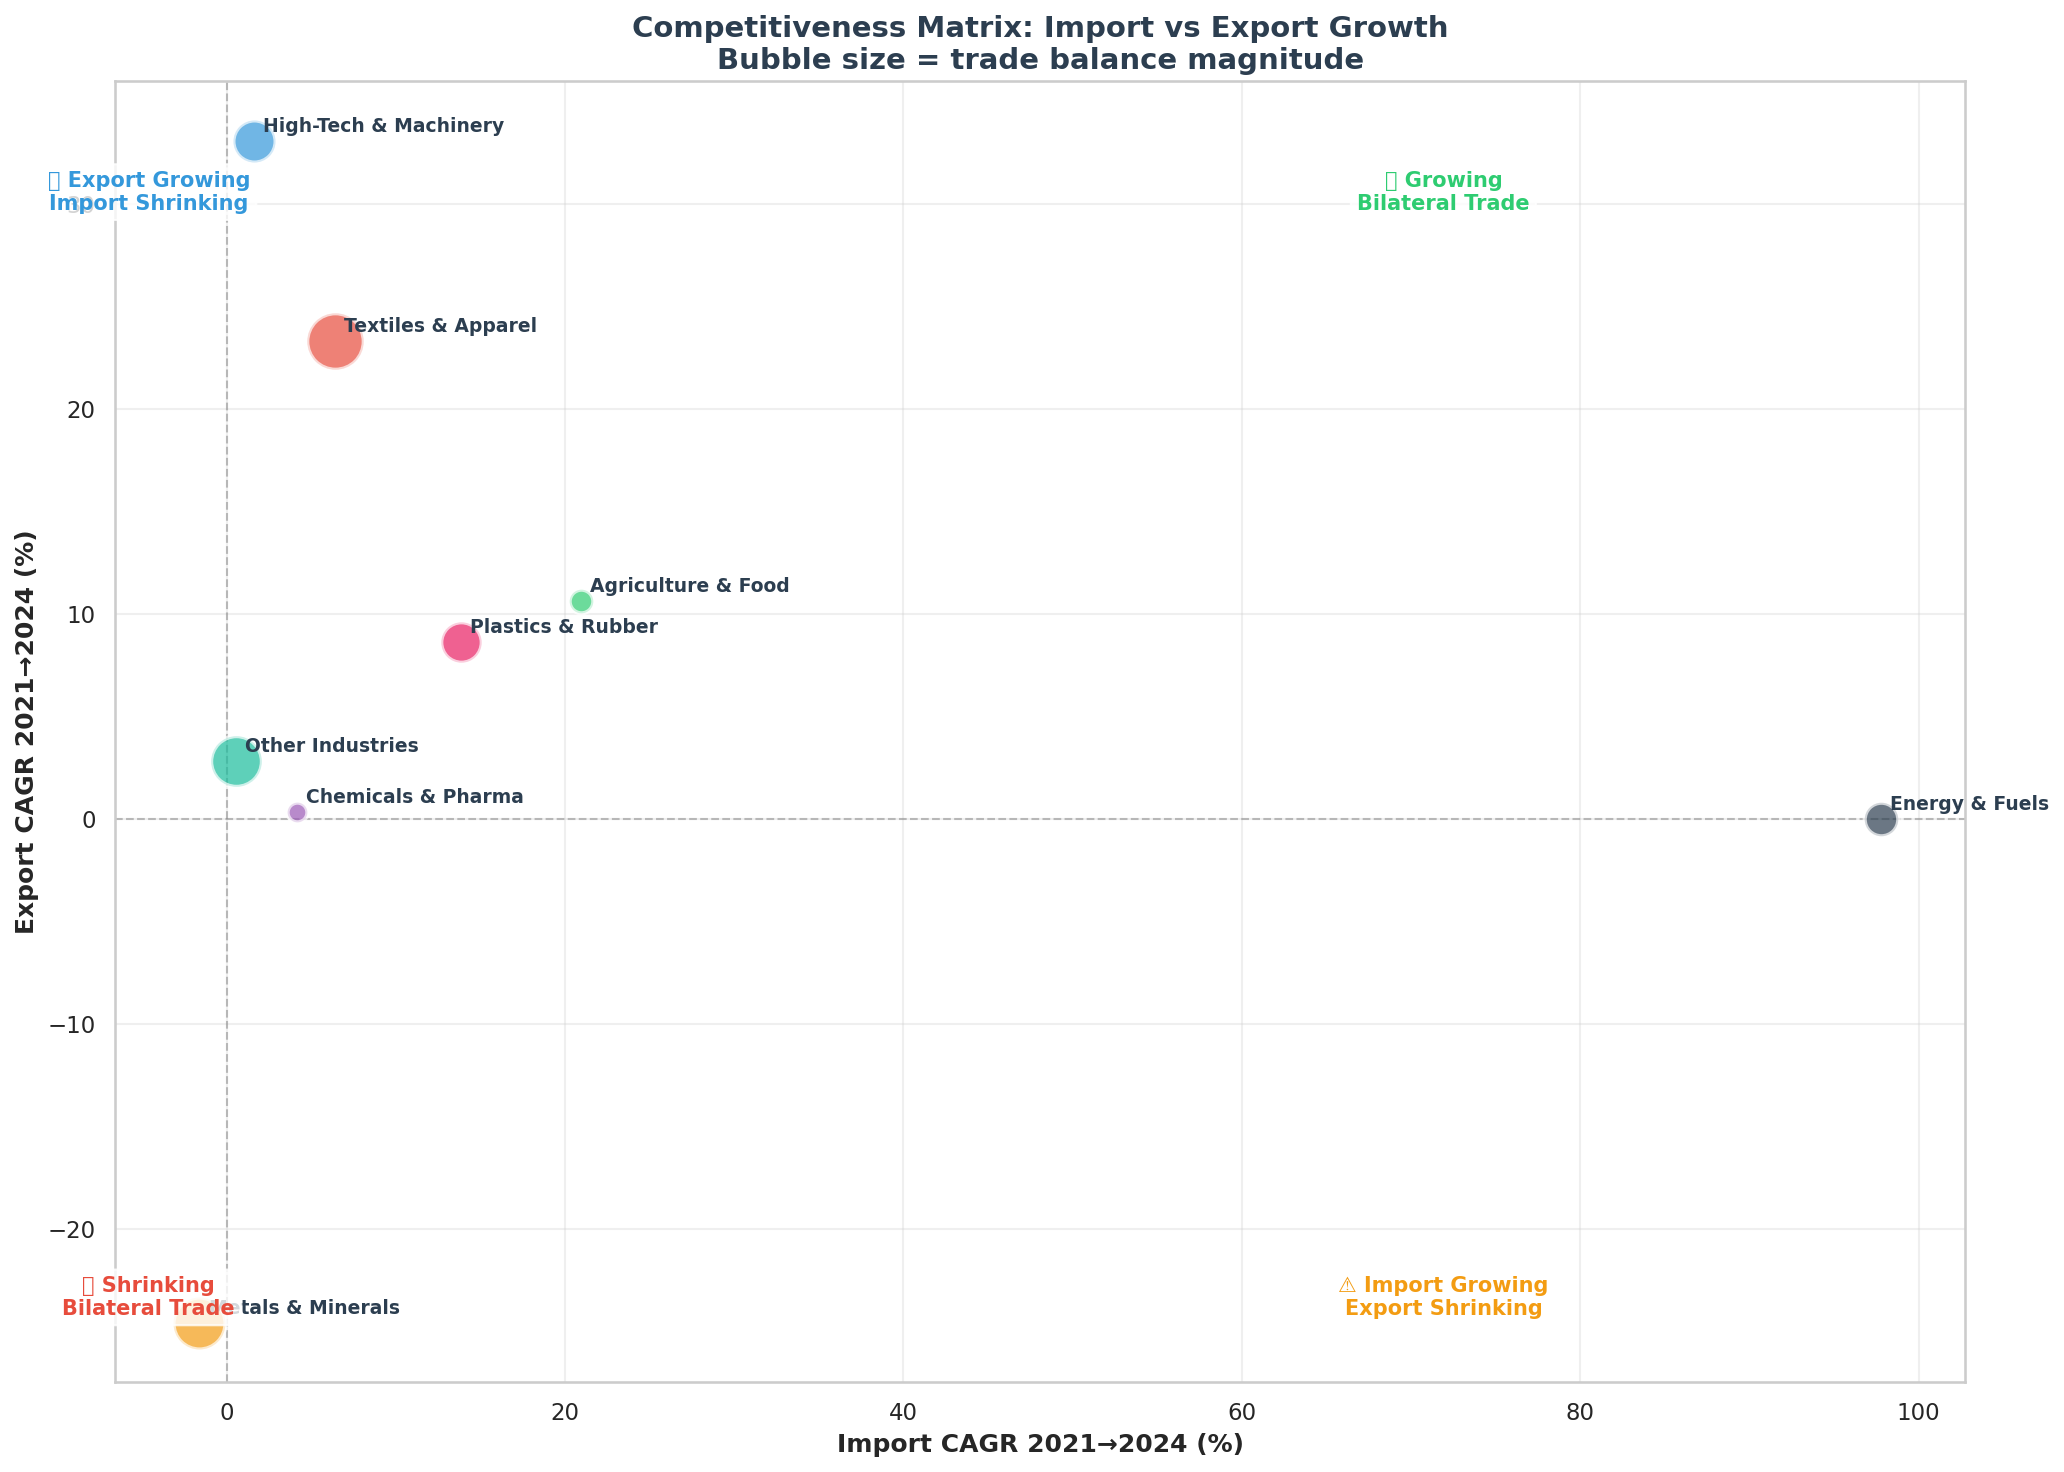
\includegraphics[width=0.95\textwidth]{../charts/19_competitiveness_matrix.png}
\caption{Competitiveness matrix plotting import CAGR vs export CAGR. Ideal position is upper-left (exports growing, imports shrinking).}
\end{figure}

The competitiveness matrix reveals four quadrants:
\begin{itemize}
\item \textbf{Upper-right (Growing bilateral trade):} Both imports and exports increasing
\item \textbf{Upper-left (Export growing, import shrinking):} Ideal position --- Morocco gaining ground
\item \textbf{Lower-right (Import growing, export shrinking):} Alarming --- widening deficit
\item \textbf{Lower-left (Both shrinking):} Declining bilateral trade
\end{itemize}

\subsection{Trade Deficit Waterfall}

\begin{figure}[H]
\centering
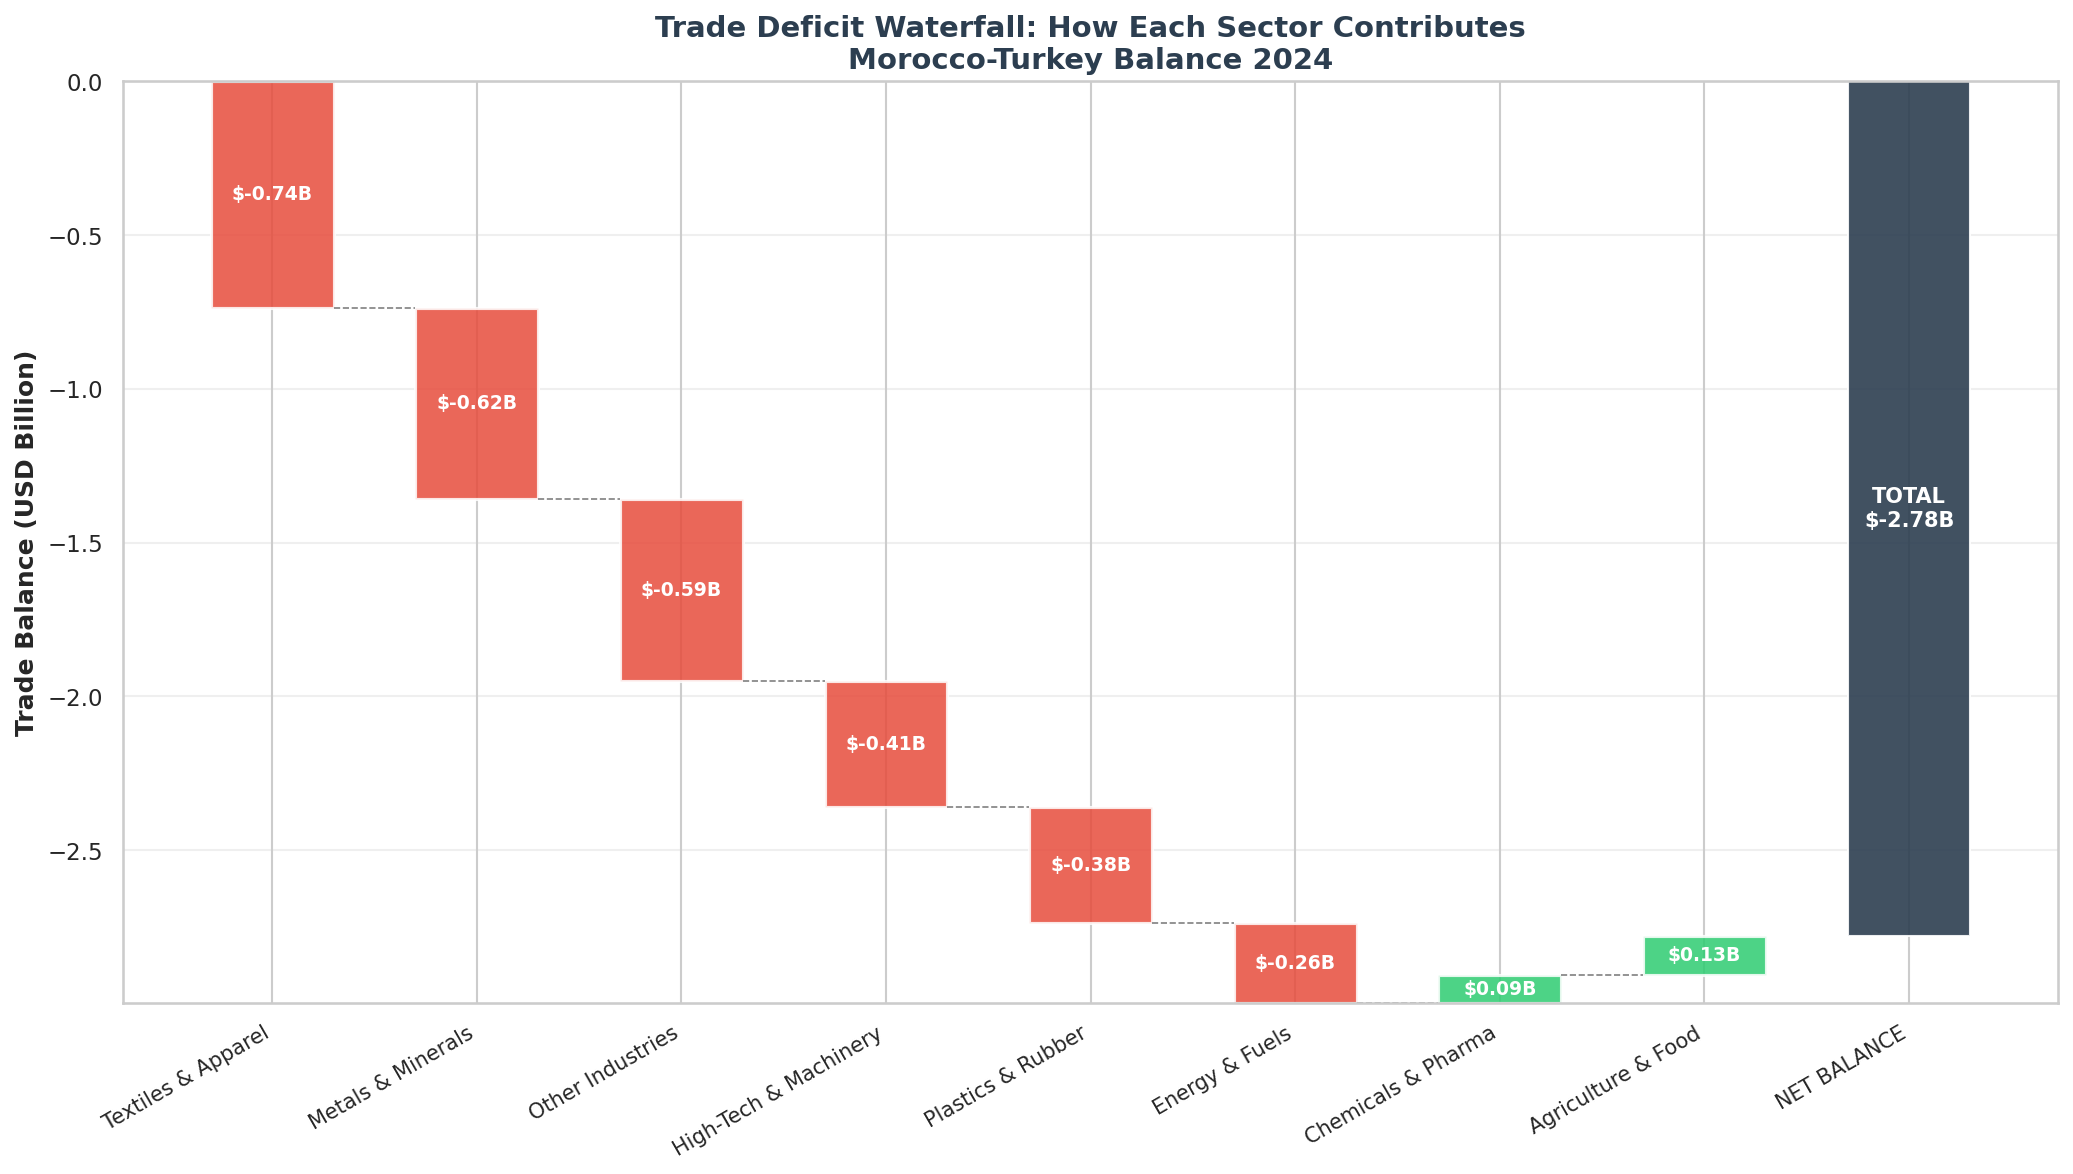
\includegraphics[width=0.95\textwidth]{../charts/18_waterfall_deficit.png}
\caption{Waterfall chart showing how each sector contributes to the overall trade deficit. Red bars are deficit sectors, green bars are surplus sectors.}
\end{figure}

\subsection{Strategic Opportunities}

\begin{figure}[H]
\centering
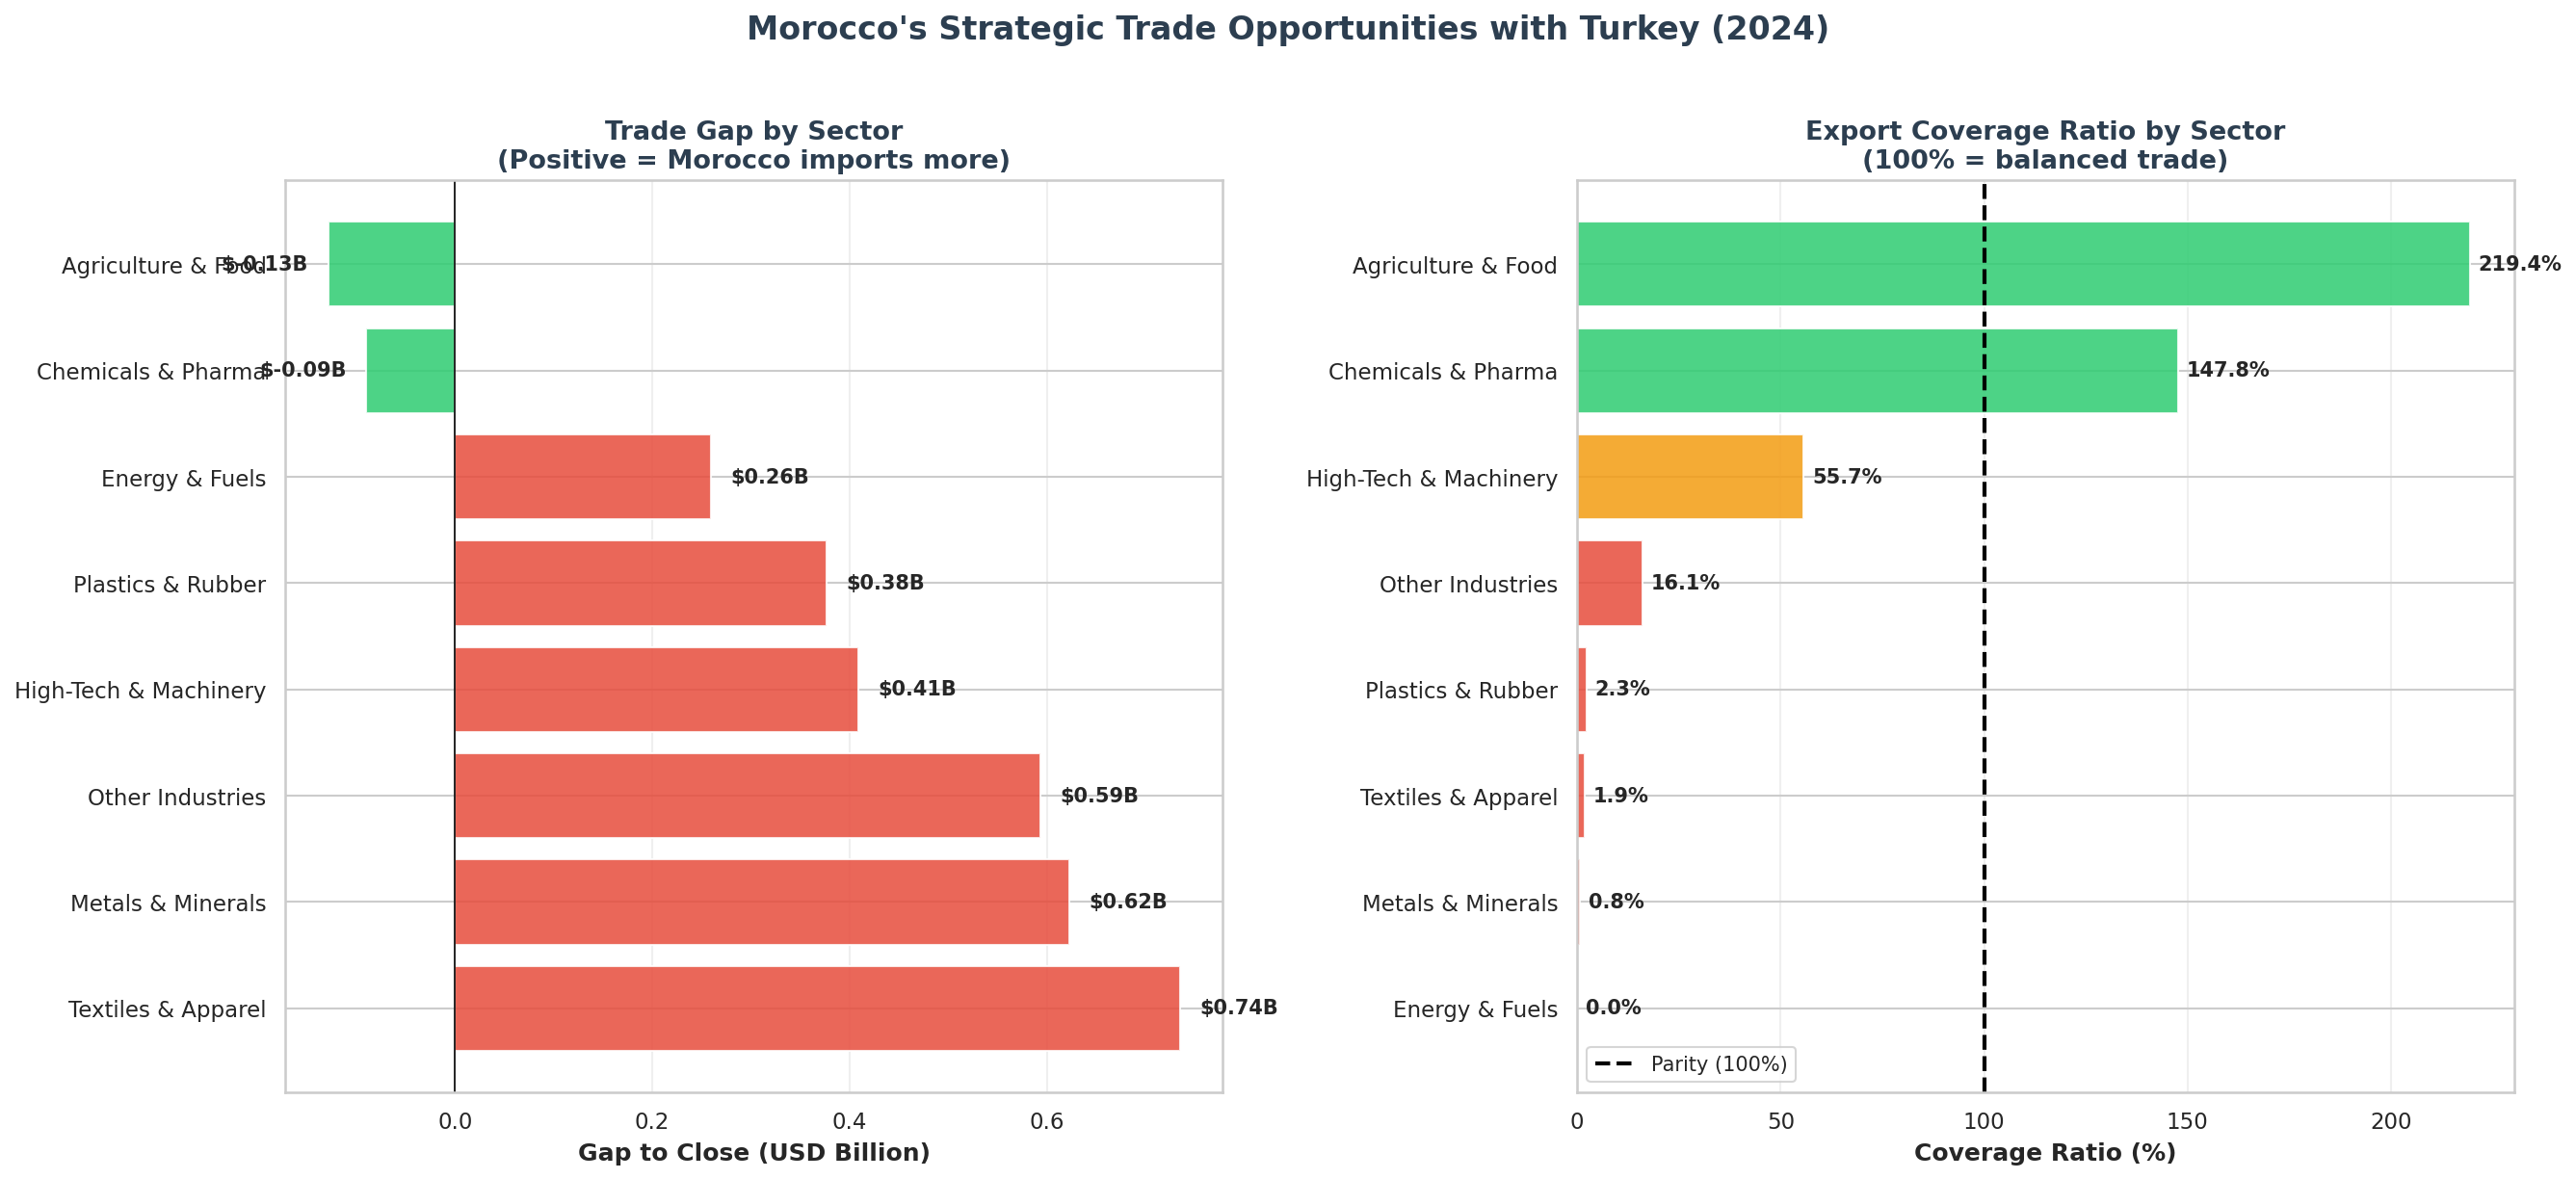
\includegraphics[width=0.95\textwidth]{../charts/20_opportunity_analysis.png}
\caption{Opportunity analysis: trade gap by sector (left) and export coverage ratio (right). Sectors with large gaps represent the biggest opportunities for import substitution.}
\end{figure}

\subsection{High-Tech Gap}

\begin{figure}[H]
\centering
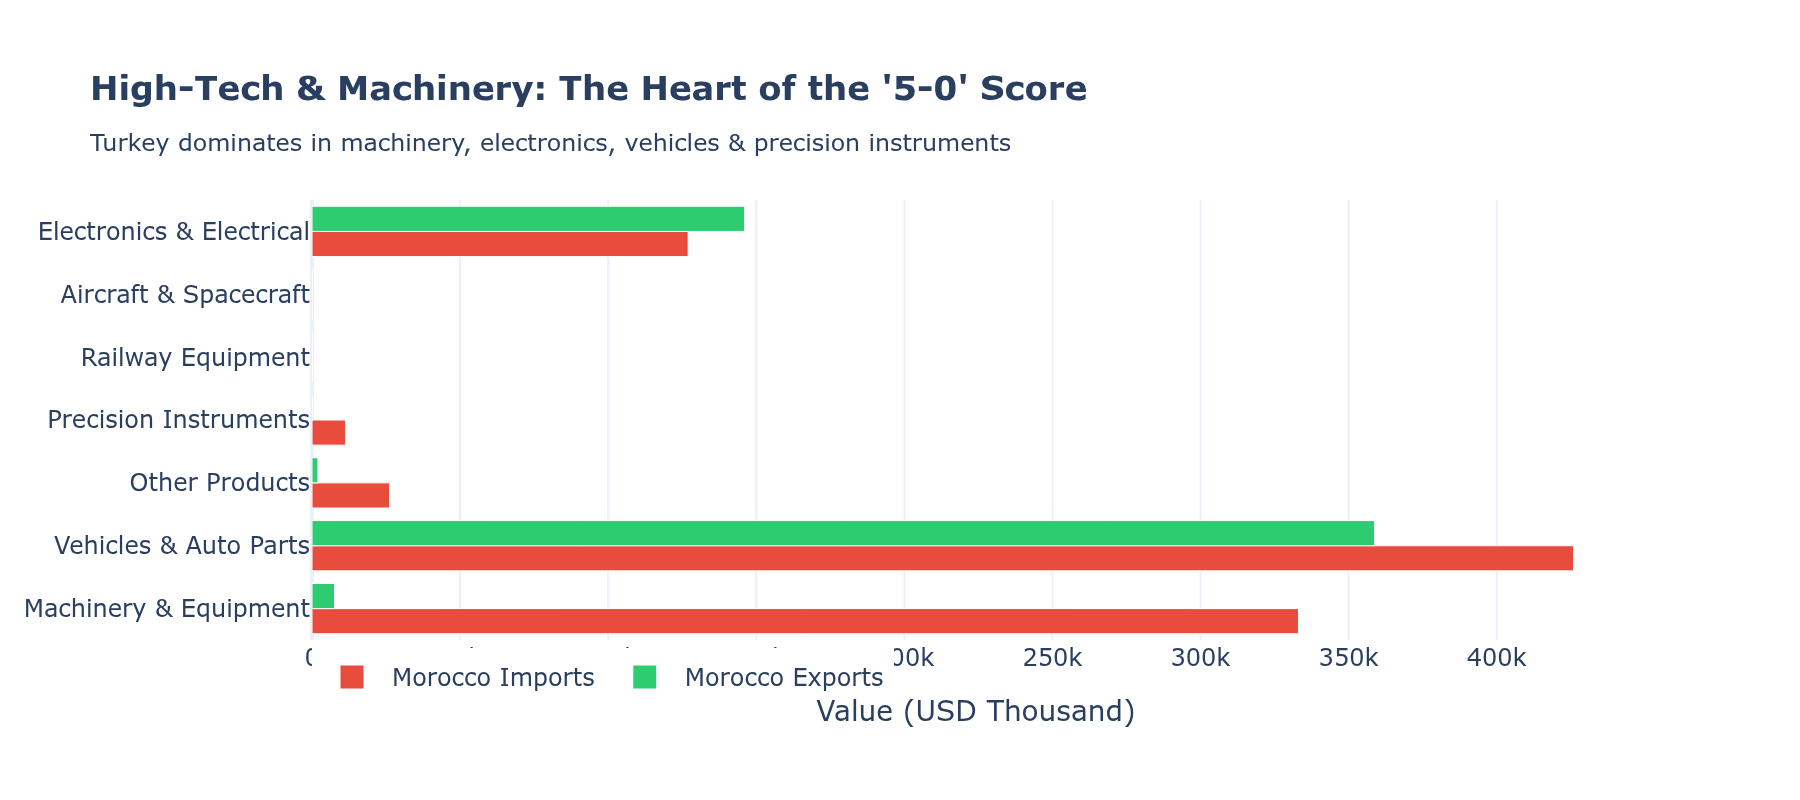
\includegraphics[width=0.95\textwidth]{../charts/13_hightech_gap.png}
\caption{Analysis of the high-tech sector gap between Morocco and Turkey, a critical area for industrial development.}
\end{figure}

\subsection{Deficit vs Surplus Products}

\begin{figure}[H]
\centering
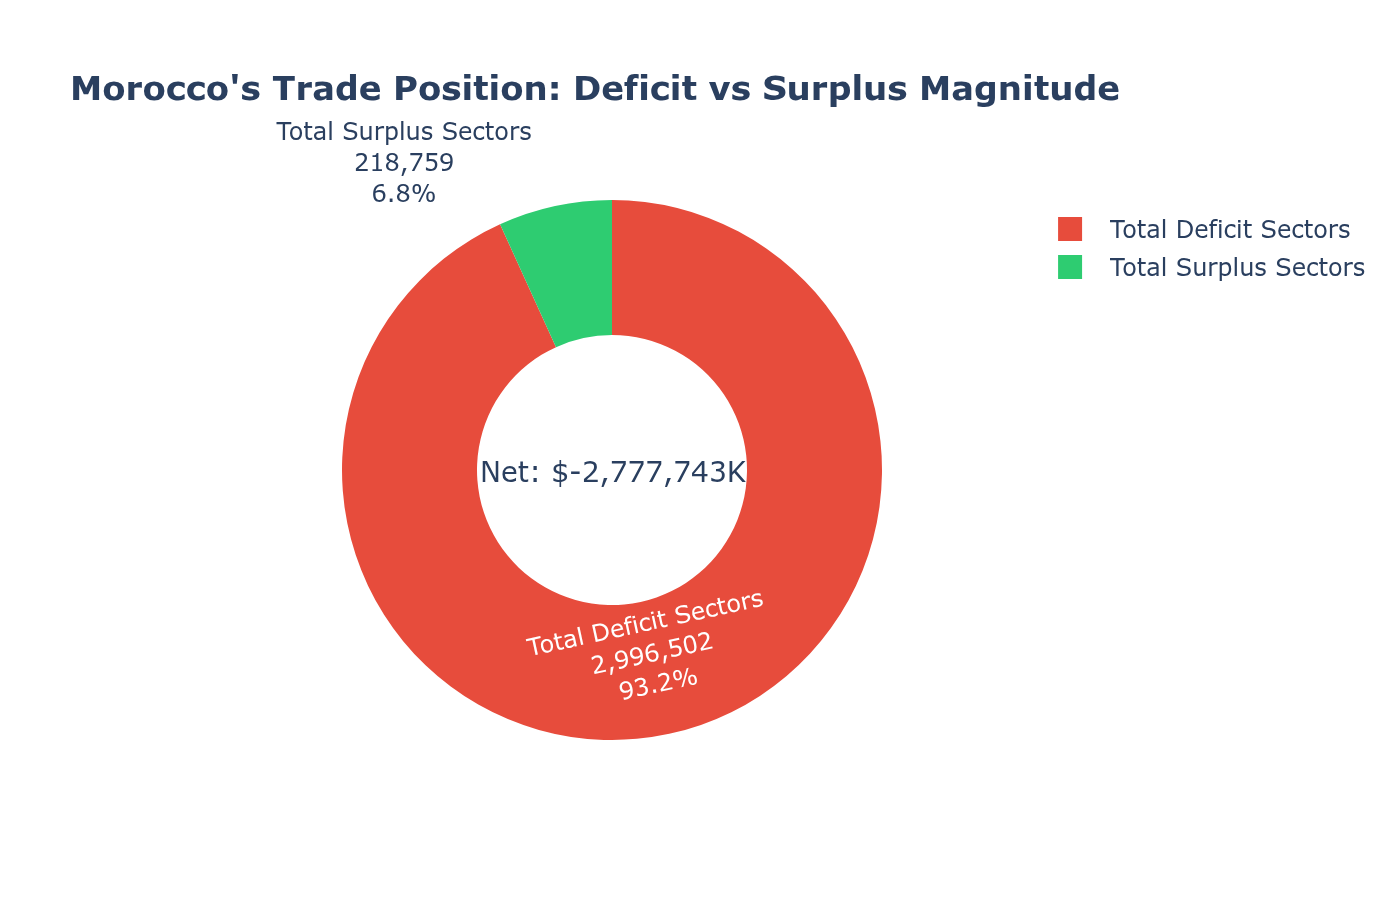
\includegraphics[width=0.95\textwidth]{../charts/15_deficit_vs_surplus.png}
\caption{Distribution of products by trade balance, showing the asymmetry between deficit and surplus categories.}
\end{figure}

% ============================================================
% 10. EXECUTIVE DASHBOARD
% ============================================================
\section{Executive Dashboard}

\begin{figure}[H]
\centering
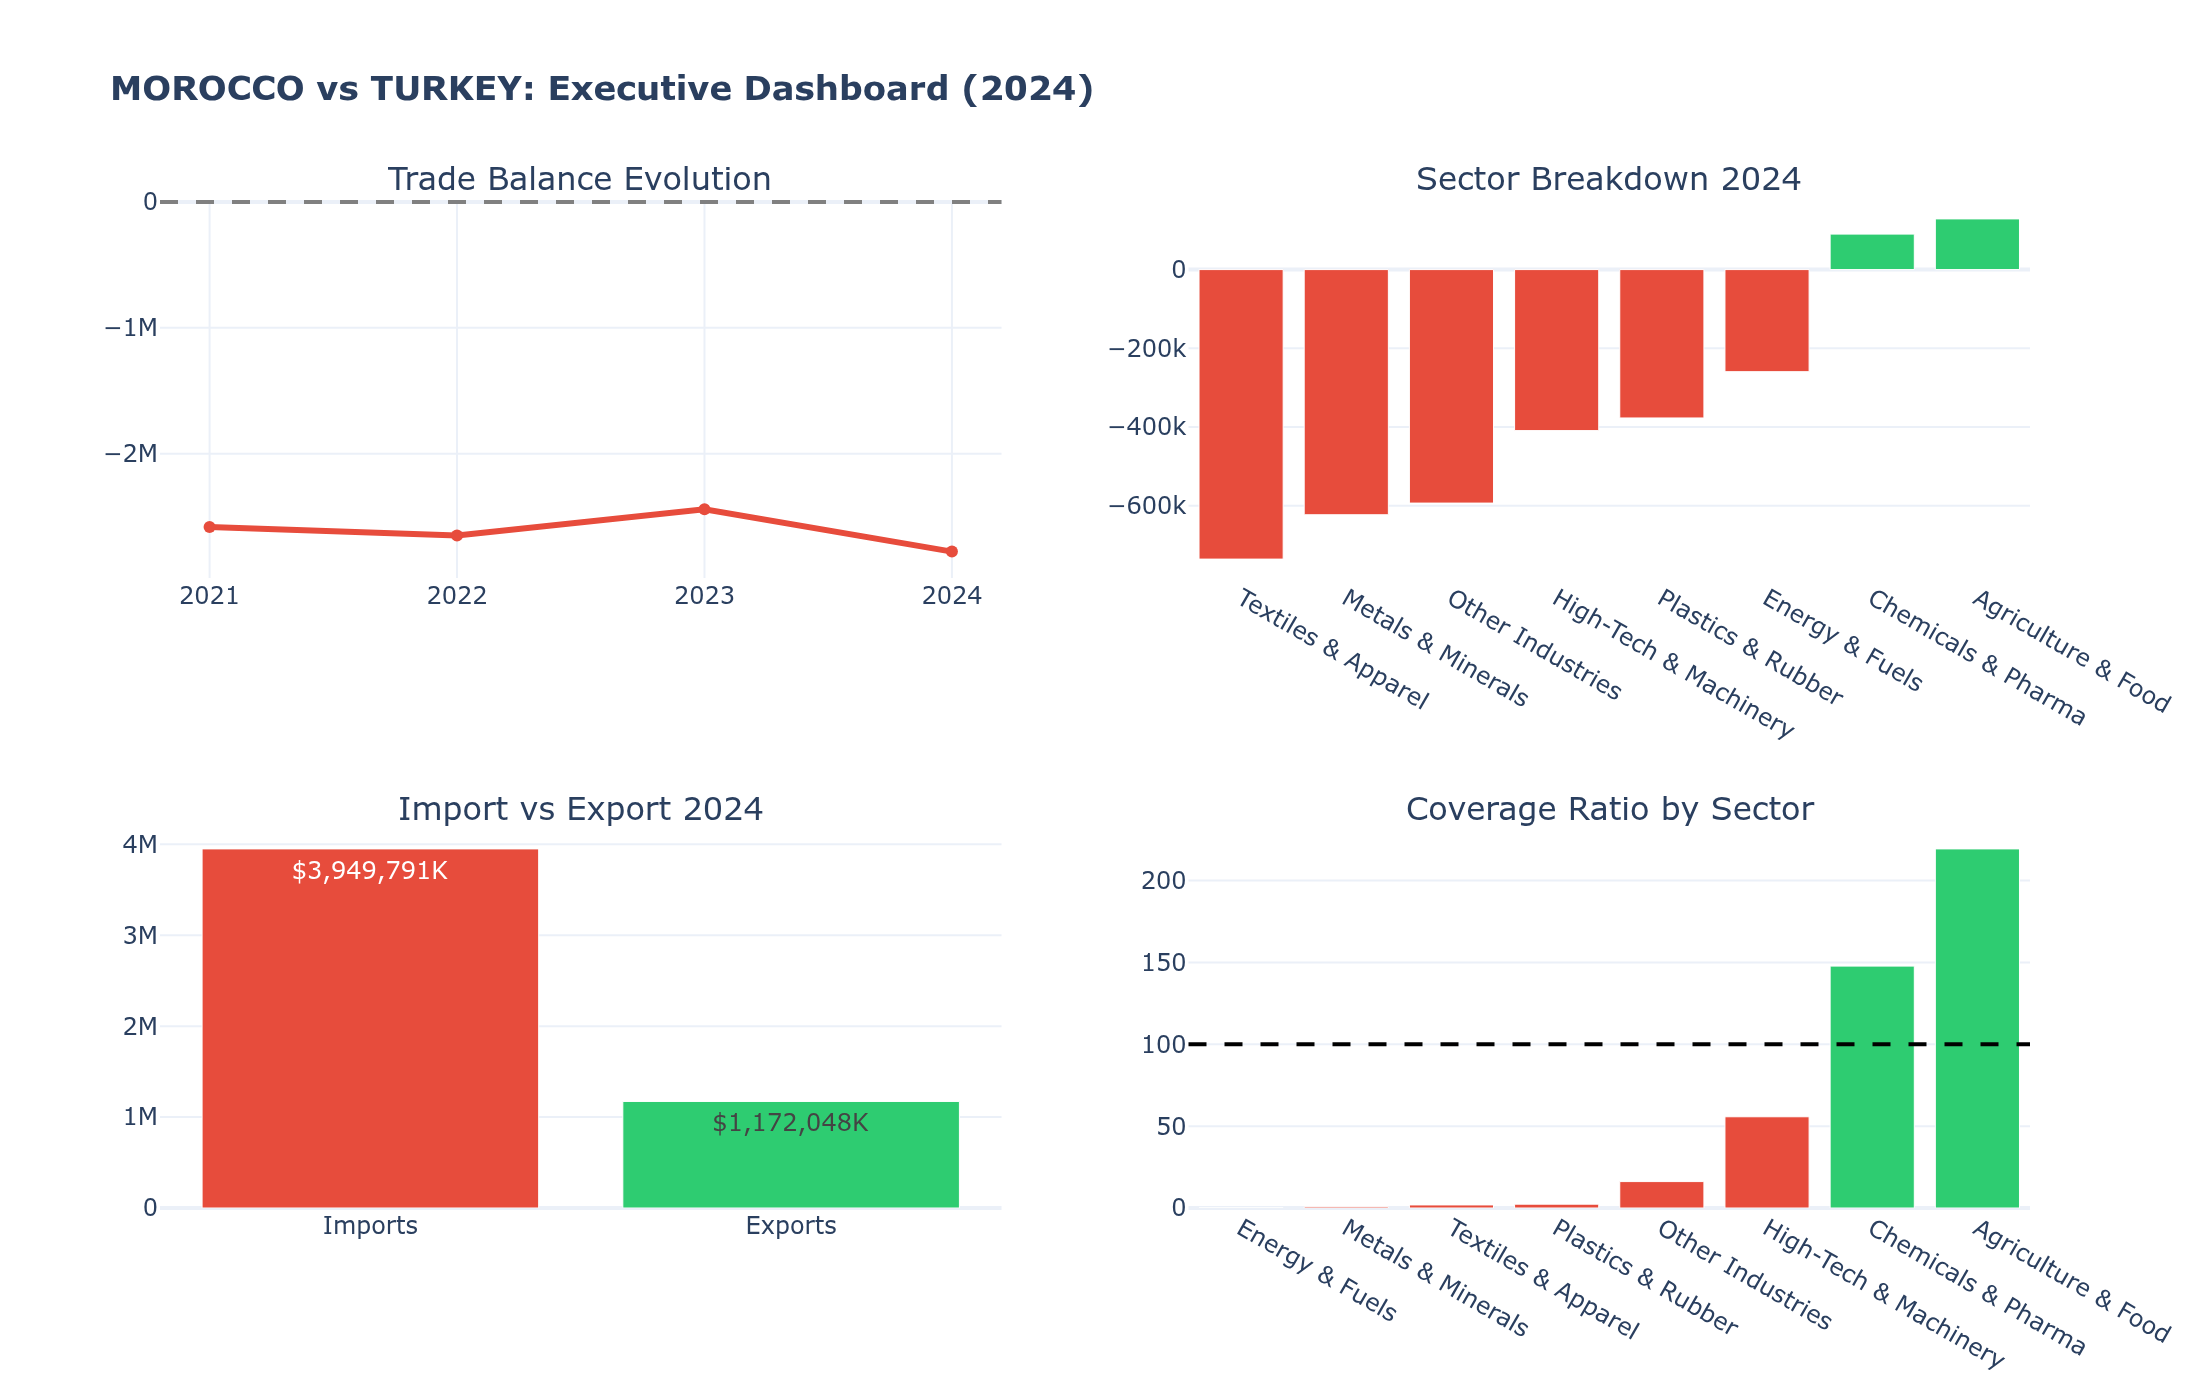
\includegraphics[width=0.95\textwidth]{../charts/16_executive_dashboard.png}
\caption{Comprehensive executive dashboard summarizing all key metrics and trends in a single view.}
\end{figure}

% ============================================================
% 11. STRATEGIC RECOMMENDATIONS
% ============================================================
\section{Strategic Recommendations}

Based on our analysis, we propose the following strategic actions:

\subsection{Short-Term Actions (1--2 Years)}

\begin{enumerate}[label=\arabic*.]
\item \textbf{Leverage existing strengths:} Scale up exports in Agriculture \& Food and Chemicals \& Pharma, where Morocco already has surpluses and established RCA.
\item \textbf{Accelerate High-Tech exports:} With a CAGR of 33.1\%, the High-Tech \& Machinery sector shows the fastest export growth. Support this momentum with targeted industrial policy.
\item \textbf{Textiles recovery:} Export CAGR of 23.3\% shows potential. Invest in vertical integration and high-value-added textile segments.
\end{enumerate}

\subsection{Medium-Term Actions (3--5 Years)}

\begin{enumerate}[label=\arabic*.]
\item \textbf{Import substitution:} Focus on Plastics \& Rubber and Other Industries where domestic capacity can realistically replace Turkish imports.
\item \textbf{Diversify exports:} Reduce HHI concentration (currently 1,589) by developing new export product categories.
\item \textbf{Automotive sector:} Leverage the Tangier Free Zone and Stellantis/Renault investments to increase automotive component exports to Turkey.
\end{enumerate}

\subsection{Long-Term Vision (5+ Years)}

\begin{enumerate}[label=\arabic*.]
\item \textbf{Match Turkey's ambition:} Turkey's trade strategy targets \$1 trillion in trade by 2030. Morocco needs an equally ambitious industrial roadmap.
\item \textbf{Africa as multiplier:} Use the African Continental Free Trade Area (AfCFTA) to build scale that enables competitiveness against Turkey in third markets.
\item \textbf{Technology transfer:} Establish joint ventures with Turkish firms to capture knowledge and technology while building domestic capacity.
\end{enumerate}

% ============================================================
% 12. CONCLUSION
% ============================================================
\section{Conclusion}

The Minister's ``5-0'' metaphor is grounded in reality: Morocco's trade deficit with Turkey stands at \$2.78 billion, with a coverage ratio of only 29.7\%. Turkey exports 3.4 times more to Morocco than it imports.

However, the data reveals reasons for cautious optimism:

\begin{itemize}
\item Morocco's export CAGR (13.6\%) is \textbf{2.6 times faster} than import growth (5.3\%)
\item The High-Tech sector is experiencing explosive export growth (+33.1\% CAGR)
\item Morocco has clear comparative advantages in 14 product categories
\item Two sectors (Agriculture and Chemicals) already show trade surpluses
\end{itemize}

The challenge is not capability --- it is, as the Minister suggested, \textbf{ambition and scale}. Morocco has the talent, the education, and the strategic position. What is needed is a systematic effort to convert these advantages into trade competitiveness, not just in a market of 30 million, but in the market of 3 billion that the Minister has opened.

\vspace{1cm}
\begin{center}
\textit{``Mesdames et messieurs, c'est fini les vacances.''}\\
--- The Minister of Industry
\end{center}

% ============================================================
% APPENDIX
% ============================================================
\newpage
\appendix
\section{Appendix: Complete Chart Index}

\begin{table}[H]
\centering
\caption{List of All 21 Charts Generated}
\begin{tabular}{c l}
\toprule
\textbf{\#} & \textbf{Chart Description} \\
\midrule
1 & Trade Evolution (2021--2024) \\
2 & Sector Balance 2024 \\
3 & The ``5-0'' Score Visualization \\
4 & Deficit Evolution \\
5 & Trade Balance Heatmap \\
6 & Top 10 Deficit Products \\
7 & Top 10 Surplus Products \\
8 & Radar Coverage by Sector \\
9 & Growth Comparison \\
10 & Import Treemap \\
11 & Export Treemap \\
12 & Dependency Index \\
13 & High-Tech Gap Analysis \\
14 & Import Composition (Pie Chart) \\
15 & Deficit vs Surplus Products \\
16 & Executive Dashboard \\
17 & CAGR by Sector \\
18 & Trade Deficit Waterfall \\
19 & Competitiveness Matrix \\
20 & Opportunity Analysis \\
21 & HHI Concentration Analysis \\
\bottomrule
\end{tabular}
\end{table}

\section{Appendix: Technical Notes}

\begin{itemize}
\item All monetary values are in US Dollars (thousands unless otherwise noted)
\item Trade data sourced from ITC Trade Map (trademap.org)
\item HS 2-digit classification used for product categorization
\item CAGR computed over 3-year period (2021 to 2024)
\item HHI computed using percentage market shares
\item RCA index uses Morocco's world export structure as reference
\item Analysis performed using Python (pandas, numpy, matplotlib, seaborn)
\item 21 professional charts generated across the analysis pipeline
\end{itemize}

\end{document}
